%%%%%%%%%%%%%%%%%%%%%%%%%%%%%%%%%%%%%%%%%
% Beamer Presentation
% LaTeX Template
% Version 1.0 (10/11/12)
%
% This template has been downloaded from:
% http://www.LaTeXTemplates.com
%
% License:
% CC BY-NC-SA 3.0 (http://creativecommons.org/licenses/by-nc-sa/3.0/)
%
%%%%%%%%%%%%%%%%%%%%%%%%%%%%%%%%%%%%%%%%%

%----------------------------------------------------------------------------------------
%	PACKAGES AND THEMES
%----------------------------------------------------------------------------------------

\documentclass{beamer}

\mode<presentation> {

% The Beamer class comes with a number of default slide themes
% which change the colors and layouts of slides. Below this is a list
% of all the themes, uncomment each in turn to see what they look like.

%\usetheme{default}
%\usetheme{AnnArbor}
%\usetheme{Antibes}
%\usetheme{Bergen}
%\usetheme{Berkeley}
%\usetheme{Berlin}
%\usetheme{Boadilla}
%\usetheme{CambridgeUS}
%\usetheme{Copenhagen}
%\usetheme{Darmstadt}
%\usetheme{Dresden}
%\usetheme{Frankfurt}
%\usetheme{Goettingen}
%\usetheme{Hannover}
%\usetheme{Ilmenau}
%\usetheme{JuanLesPins}
%\usetheme{Luebeck}
\usetheme{Madrid}
%\usetheme{Malmoe}
%\usetheme{Marburg}
%\usetheme{Montpellier}
%\usetheme{PaloAlto}
%\usetheme{Pittsburgh}
%\usetheme{Rochester}
%\usetheme{Singapore}
%\usetheme{Szeged}
%\usetheme{Warsaw}

% As well as themes, the Beamer class has a number of color themes
% for any slide theme. Uncomment each of these in turn to see how it
% changes the colors of your current slide theme.

%\usecolortheme{albatross}
%\usecolortheme{beaver}
%\usecolortheme{beetle}
%\usecolortheme{crane}
%\usecolortheme{dolphin}
%\usecolortheme{dove}
%\usecolortheme{fly}
%\usecolortheme{lily}
%\usecolortheme{orchid}
%\usecolortheme{rose}
%\usecolortheme{seagull}
%\usecolortheme{seahorse}
%\usecolortheme{whale}
%\usecolortheme{wolverine}

%\setbeamertemplate{footline} % To remove the footer line in all slides uncomment this line
%\setbeamertemplate{footline}[page number] % To replace the footer line in all slides with a simple slide count uncomment this line

%\setbeamertemplate{navigation symbols}{} % To remove the navigation symbols from the bottom of all slides uncomment this line
}

\usepackage{graphicx} % Allows including images
\usepackage{booktabs} % Allows the use of \toprule, \midrule and \bottomrule in tables
\usepackage{cool}

%----------------------------------------------------------------------------------------
%	TITLE PAGE
%----------------------------------------------------------------------------------------

\title[Agency MBS Pricing]{Towards Improved Pricing and Hedging of \\ Agency Mortgage-Backed Securities (MBS)} % The short title appears at the bottom of every slide, the full title is only on the title page

\author{Ashwin Rao} % Your name
\institute[AFTLab Seminar @ Stanford] % Your institution as it will appear on the bottom of every slide, may be shorthand to save space
{
Presentation for AFTLab Seminar at Stanford University\\ % Your institution for the title page
}

\date{\today} % Date, can be changed to a custom date

\begin{document}
\begin{frame}
\titlepage % Print the title page as the first slide
\end{frame}

\begin{frame}
\frametitle{Overview} % Table of contents slide, comment this block out to remove it
\tableofcontents % Throughout your presentation, if you choose to use \section{} and \subsection{} commands, these will automatically be printed on this slide as an overview of your presentation
\end{frame}

\section{Mortgage Basics}

\begin{frame}
\frametitle{Mortgage Basics: Borrower's Perspective}
\begin{itemize}
\item A family wants to buy a house worth \$500K
\item Can make down-payment of \$100K $\Rightarrow$ Loan to Value (LTV) of 80\%
\item Borrower has a good FICO score of 750
\item Monthly family income is \$6000, Current monthly debt is only \$100
\item So qualifies for a good mortgage rate (30 year, Fixed Rate) of 4\%
\item Monthly payment (Interest + Principal) amounts to about \$1900
\item Debt to Income (DTI) is $\frac {1900 + 100} {6000} =$ 33\%
\item {\bf Psychology less about debt mgmt, more about cash flows (DTI)}
\end{itemize}
\end{frame}

\begin{frame}
\begin{figure}
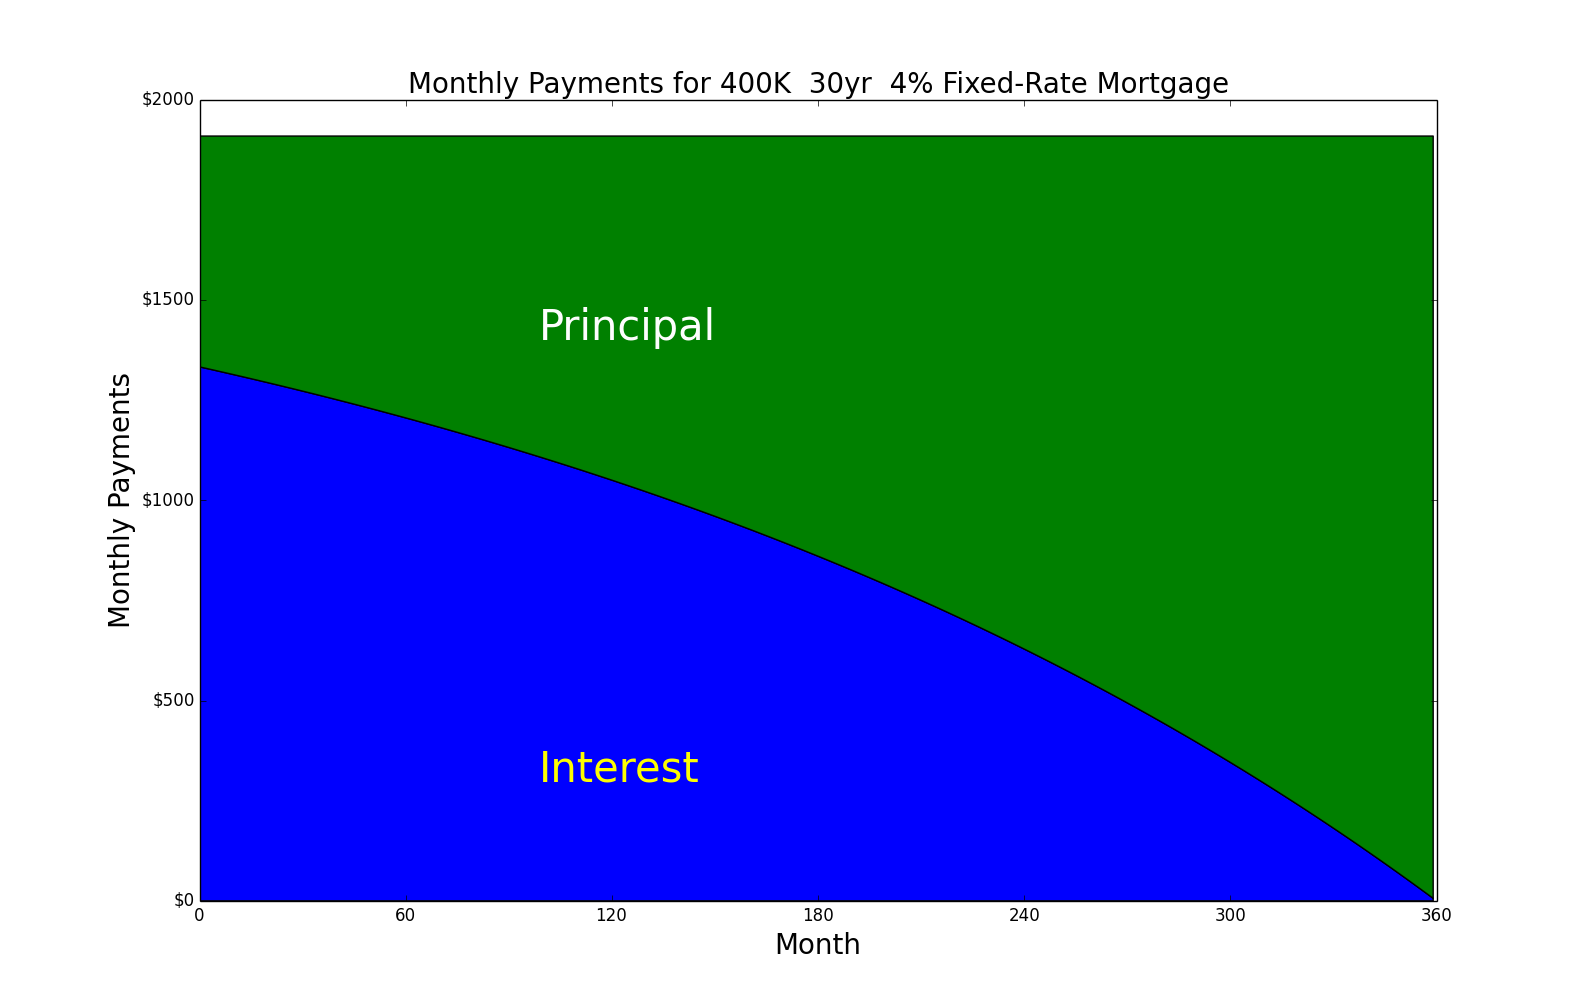
\includegraphics[scale=0.32]{monthly_pni.png}
\end{figure}
\end{frame}

\begin{frame}
\frametitle{Mortgage Basics: Lender's Perspective}
\begin{itemize}
\item The lender requires documentation on income, other assets/debts
\item The lender is long a ``Bond'' receiving monthly Principal \& Interest
\item Lender's biggest risk is the borrower defaulting on monthly payments
\item Think of this as the Borrower's (American) Put option on the House, with Strike = Remaining Principal (Default $\Rightarrow$ House taken away)
\item {\bf Lender will offer a rate commensurate with LTV, DTI, FICO}
\end{itemize}
\end{frame}

\begin{frame}
\frametitle{Lender also exposed to {\em Voluntary Prepayment} Risk}
\begin{itemize}
\item {\em Prepayment} refers to Principal being paid off before maturity
\item Borrower Defaulting is refered to as {\em Involuntary Prepayment}
\item Voluntary Prepayment mainly due to Refinancing or Home Sales
\item Think of this as the Borrower's (American) Call option on the Loan, \\ with Strike = Remaining Principal
\item In-the-money when offered rate is below rate on borrower's mortgage
\item Refinancing: Borrowers often exercise deep in-the-money (suboptimal) 
\item HomeSales: Often happens when option is out-of-the-money
\item {\bf So Prepayment Risk is a ``hard to model'' Risk}
\end{itemize}
\end{frame}

\begin{frame}
\frametitle{Value, Balance and Price}
\begin{itemize}
\item The following terms reference the Bond (loan) owned by the lender
\item {\em Value}: Present Value of future Principal and Interest payments
\item {\em Balance}: Principal that is remaining to be paid
\item {\em Price} (Quantity of Interest): {\em Value} divided by {\em Balance}
\item {\bf Prepayment option is a call option on {\em Price} with strike = 1} \\ (ignoring transaction costs)
\item Later, we will derive the PDE for {\em Price} and assess {\em Price Sensitivity}
\end{itemize}
\end{frame}

\section{Agency Securitization}

\begin{frame}
\frametitle{Agency Securitization of a Pool of Mortgages}
\begin{itemize}
\item ``Agency'' refers to the Government-sponsored entities (GSE)
\item Fannie Mae, Freddie Mac, Ginnie Mae
\item Pool of {\em Conforming} loans (conservative loan size, LTV, DTI, docs)
\item Agency receives collective Principal \& Interest from the pool
\item In Exchange for cash extended to banks to originate mortgages
\item Agency issues a Mortgage-Backed Security (backed by mortgage pool)
\item Passthrough MBS simply forwards mortgage cash flows to investors
\end{itemize}
\end{frame}

\begin{frame}
\frametitle{Some details of Agency MBS}
\begin{itemize}
\item ``Servicer'' responsible for collection of payments from borrowers
\item Servicer receives a servicing fee for the service it provides
\item Conforming loans $\Rightarrow$ risk of borrower delinquencies/default is low
\item Agency guarantees investors principal even when a borrower defaults
\item Defaulted loan is taken out of pool, investor receives {\bf full principal}
\item So Agency MBS investor has {\bf no credit-risk} (government backing!)
\item Agency receives a guarantee fee for this credit protection
\item Guarantee fee + Servicing fee $\approx$ 50bp of Pool Balance
\item So MBS coupon $\approx$ 50bp less than Pool's Average Mortgage Rate 
\end{itemize}
\end{frame}


\begin{frame}
\frametitle{Agency MBS securitized from a Conforming Pool of Loans}
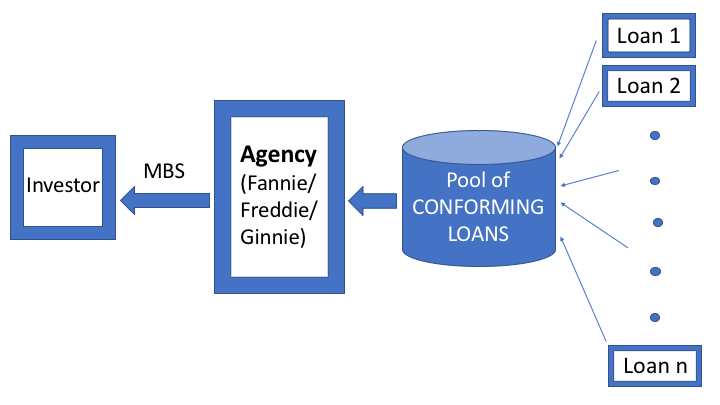
\includegraphics[scale=0.35]{securitization_flow.png}
\end{frame}

%\begin{frame}
%\begin{figure}
%\includegraphics[scale=0.75]{AgencySecuritization.png}
%\end{figure}
%\end{frame}


\begin{frame}
\frametitle{Investor Perspective of Prepayment Risk for Passthroughs}
\begin{itemize} 
\item Investor requires compensation for being short the Prepayment Option
\item Prepayments for Premiums (Price $>1$) are mainly Refinancings
\item Prepayments for Discounts (Price $<1$) are mainly HomeSales
\begin{itemize}
\item Price for a Premium reduces when Prepayments rise
\item Price for a Discount increases when Prepayments rise
\item Price for the Par Passthrough is insensitive to Prepayments
\end{itemize}
\end{itemize}
\end{frame}

\begin{frame}
\frametitle{Investor Perspective of Hedging Passthroughs}
\begin{itemize}
\item Duration Definition: $-\frac {1} {P} \pderiv{P}{r}$
\item Duration viewed as cashflows-PV-weighted average time of cash flows
\item Duration is lower when Price is higher
\item Duration reduces when Prepayments rise
\item Short Prepayment Option $\Rightarrow$ Convexity and Vega are negative
\end{itemize}
\end{frame}

\begin{frame}
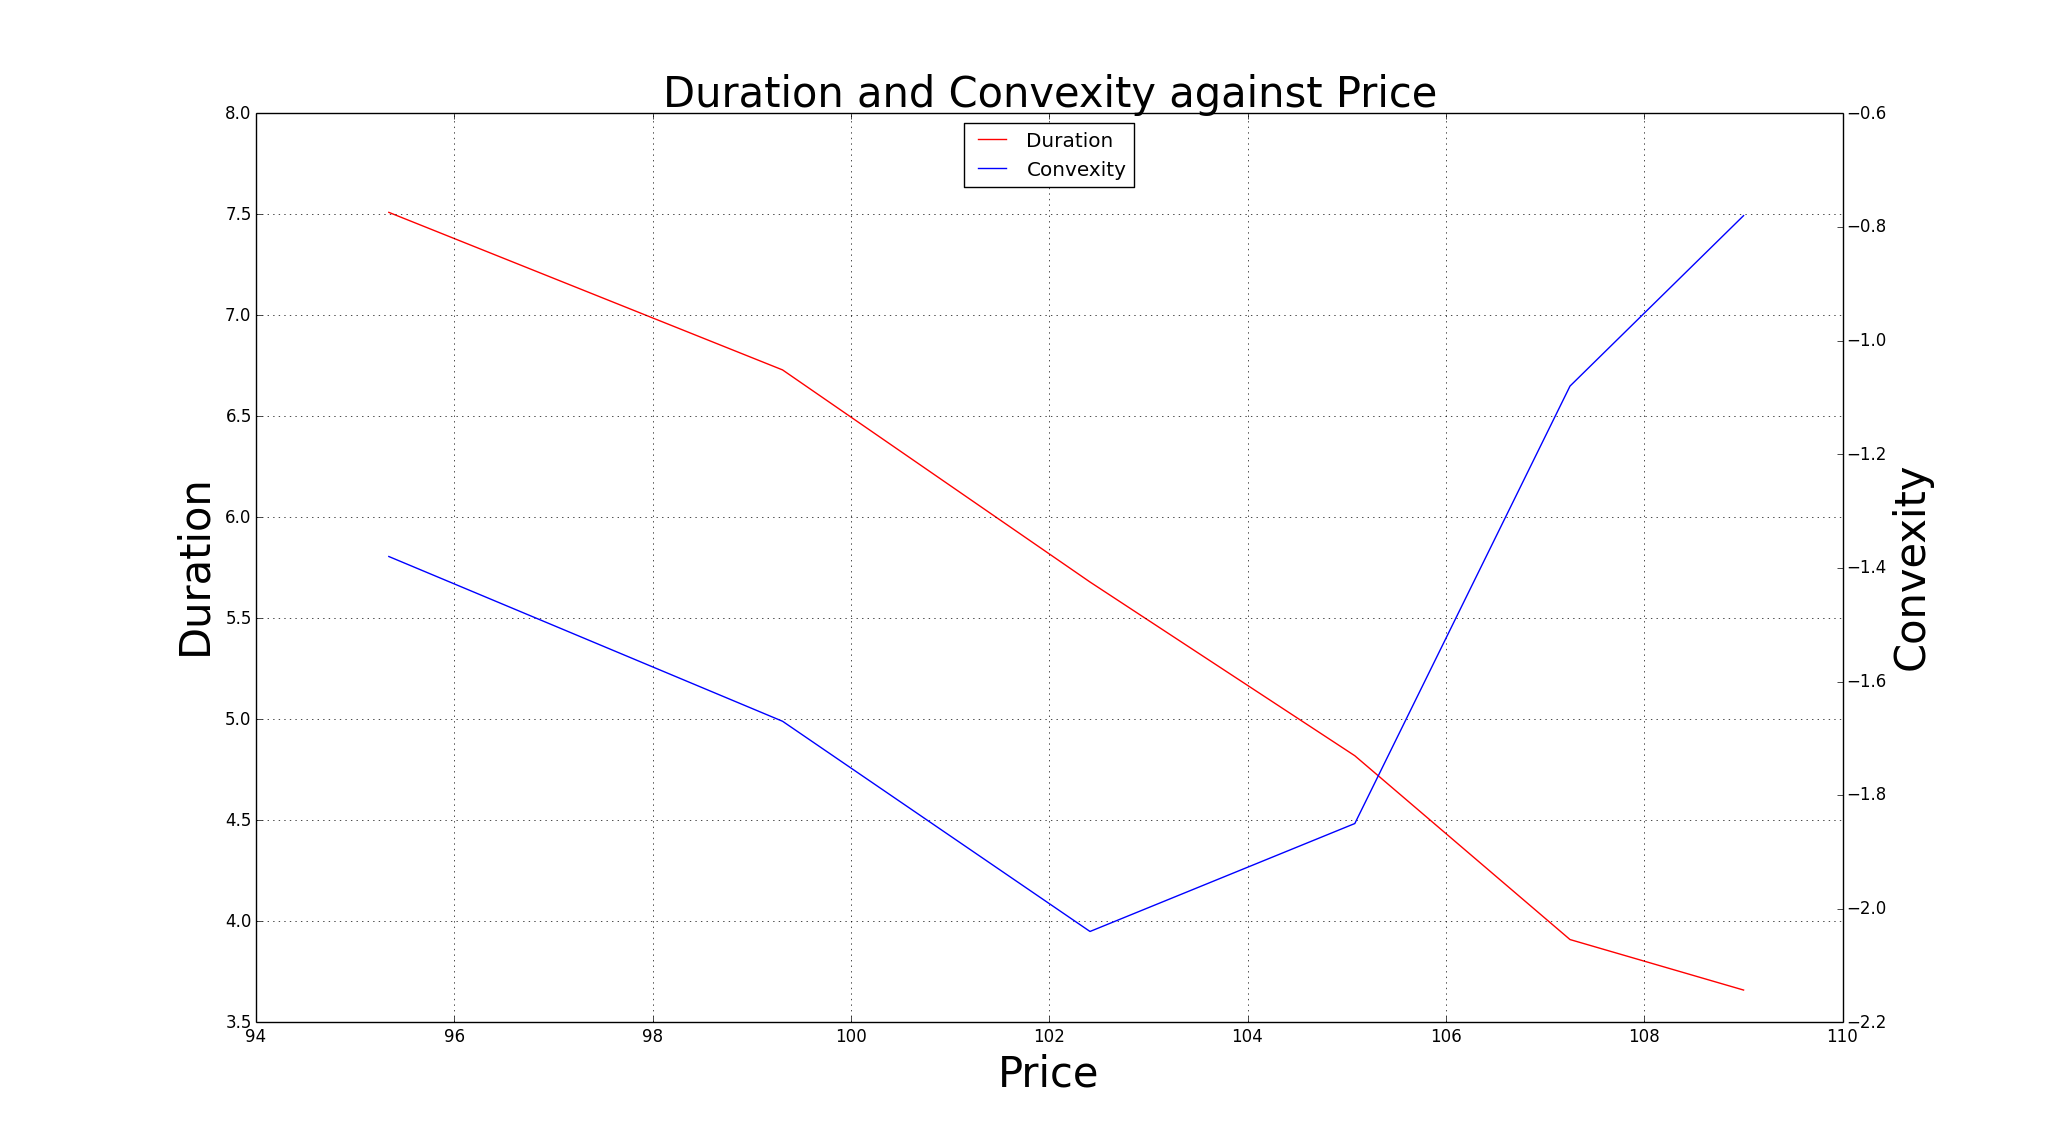
\includegraphics[scale=0.24]{dur_conv_against_price.png}
\end{frame}

\section{Structuring}

\begin{frame}
\frametitle{Structuring}
\begin{itemize}
\item Pro Rata Structuring
\item Sequential Pay Tranches
\item Planned Amortization Class (PAC) Tranches
\end{itemize}
The key rule in structuring is that the sum of principal cash flows to the tranches equals the principal cash flows in the collateral (even if one or more of the tranches gets ``negative'' principal payments, eg: Z-Tranche), and likewise for the sum of interest cash flows.
\end{frame}

\begin{frame}
\frametitle{Pro Rata Structuring}
\begin{itemize}
\item Proportional Principal flows for each security but different coupons 
\item Floaters
\item Inverse Floaters
\item Interest Only (IO)
\item Principal Only (PO)
\item Inverse Interest Only (IIO)
\end{itemize}
\end{frame}

\begin{frame}
\frametitle{Sequential Pay Tranches}
\begin{itemize}
\item All Principal flows to Senior-most tranche until it is paid down
\item After which all principal flows to the next tranche and so on ... 
\item Duration of tranches sorted by tranche seniority
\item A particularly exotic structure: Z-Accrual Tranching
\begin{itemize}
\item Junior Tranche is known as the Z-Accrual Tranche
\item Senior Tranche receives interest of Junior Tranche as principal
\item Meanwhile, Junior Tranche accrues its interest as principal
\item When Senior is paid off, Junior receives both principal \& interest
\end{itemize}
\end{itemize}
\end{frame}

\begin{frame}
\frametitle{Planned Amortization Class (PAC) Tranches}
\begin{itemize}
\item Simplest Structure: 1 PAC Tranche and 1 Support Tranche
\item We set two deterministic prepayment schedules $S_H$ and $S_L$
\item PAC receives minimum of principal payments of $S_H$ and $S_L$
\item Any excess principal flow will go to the Support Tranche
\item Thus, PAC principal payments are deterministic and so, low-risk
\item Except when prepayments get extremely low or extremely high
\item Extremely high prepayments can result in Support getting paid down
\item Support Tranche absorbs most of the prepayment risk
\end{itemize}
\end{frame}

\section{Industry-Standard approach to Pricing \& Hedging}

\begin{frame}
\frametitle{Industry-Standard approach to Pricing \& Hedging}
The components of a typical Agency MBS Pricing/Hedging System
\begin{itemize}
\item Stochastic interest rate model calibrated to liquid rate/vol instruments
\item Monte Carlo simulation of interest rate model
\item Econometric model of prepayments
\item Regression model of mortgage rates (function of interest rates)
\item Cash flow generator for various MBS Structures
\item Pricing/Sensitivities based on notion of ``Option-Adjusted Spread''
\end{itemize}
\end{frame}


\begin{frame}
\frametitle{Interest Rate Model}
\begin{itemize}
\item Calibration to liquid rate/vol instruments
\item Multi-factor model needed to capture non-parallel curve moves
\item Capturing Vol Skew/Smile very important for MBS
\item So need to also calibrate to OTM swaptions' market vol
\item Model Choices: Local Vol, Stochastic Vol, CEV, Jump Diffusion
\item Short rate or Markovian HJM models typically prefered
\end{itemize}
\end{frame}

\begin{frame}
\frametitle{Monte-Carlo Simulation}
\begin{itemize}
\item Two reasons for needing to do non-Markovian Pricing of MBS:
\begin{itemize}
\item Burnout modeling (can be made Markovian, as explained later)
\item Many CMOs have cash flows that depend on history of cash flows
\end{itemize}
\item Sequence of draws of Brownian increments gives a path of states 
\item This provides discount factors at each time step
\item For cash flows, need analytic/grid mapping from State to Rates/Vols
\item Variance reduction:
\begin{itemize}
\item Antithetic variables ($E[dz_t] = 0$ for all $t$)
\item Ensure $E[(dz_t)^2] = dt, E[(dz_s)(dz_t)] = 0$ using Orthonormalization
\item Control Variates, Quasi Random Numbers, Brownian Bridge
\end{itemize}
\end{itemize}
\end{frame}


\begin{frame}
\frametitle{Prepayment Modeling}
\begin{itemize}
\item Goal: Estimating the probability of loan termination
\item Using information on loan/borrower/collateral/economic conditions
\item Prepayment (Loan Termination) can be due to:
\begin{itemize}
\item HomeSales (typically job-related or buying more expensive house)
\item Refinancing (to get a lower rate, or for cash-out refinance)
\item Default ($\Rightarrow$ loan paid off and removed from pool)
\item Curtailment (partial prepayment to curtail the life of the loan)
\end{itemize}
\item Most prepayments for agency loans are home sales and refinancings
\end{itemize}
\end{frame}

\begin{frame}
\frametitle{Homogeneity of Loans in Agency Pool $\Rightarrow$ Pool-Level Model}
\begin{itemize}
\item Homogeneous in loan age, coupon, loan size, underwriting standards
\item So, industry-standard is pool-level modeling (with some adjustments)
\item Predicts fraction of pool terminating under given economic scenario
\item Statistical model with modeler-imposed regressors \& functional forms
\item Recent advances in Deep Learning technology {\bf should be exploited}
\item Loan-level data has been made available recently that is useful to address non-homogeneity of credit quality of loans
\item Though investor has no credit risk, borrower credit affects incentive to refinance/sell, and likelihood of default-based termination
\end{itemize}
\end{frame}

\begin{frame}
\frametitle{Economic Intuition of HomeSales Model}
\begin{itemize}
\item HomeSales volume varies significantly by different seasons of the year
\item Ramp up in home sales as a function of loan age
\item Higher home prices leads to homeowners ``trading up''
\item Higher credit borrowers face less frictions
\item ``Lock-in'' effect: Borrowers with low mortgage rate (relative to offered rate) reluctant to move as they like to hold on to their low rate
\end{itemize}
\end{frame}

\begin{frame}
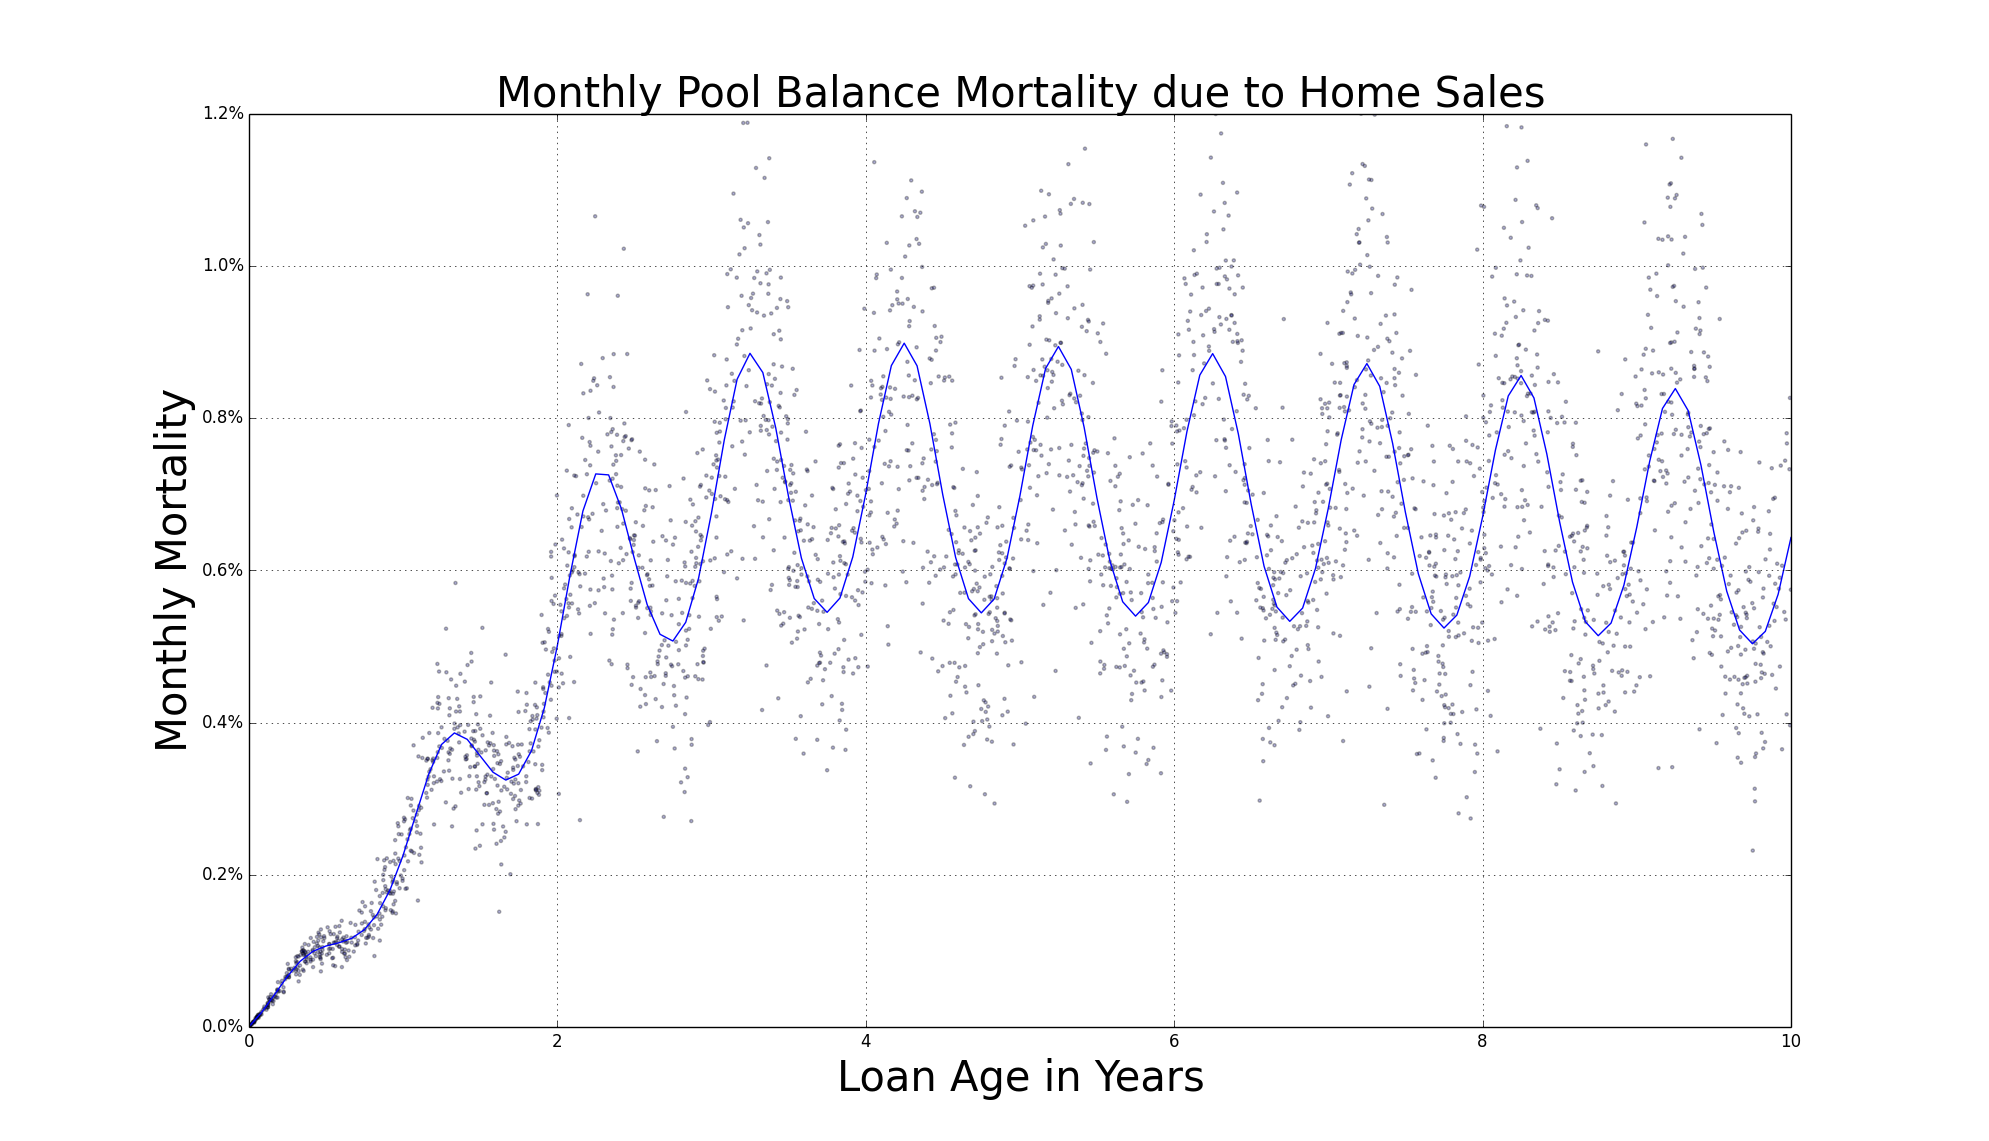
\includegraphics[scale=0.26]{relo_by_age.png}
\end{frame}

\begin{frame}
\frametitle{Economic Intuition of Refinancing Model}
\begin{itemize}
\item Incentive is typically the \% improvement in monthly payments
\item Mortgage Rate difference (``moneyness'') is used as an approximation
\item Lower credit quality diminishes the ability to refinance
\item Credit quality indicators are SATO, FICO, LTV, DTI, Home Prices
\item Higher home prices lead to cash-out refinancing
\item Burnout Effect (Heterogeneity in borrower refinancing efficiency)
\item Opportunity to make Refinancing model Markovian by creating cohorts homogeneous in their refinancing efficiency
\end{itemize}
\end{frame}

\begin{frame}
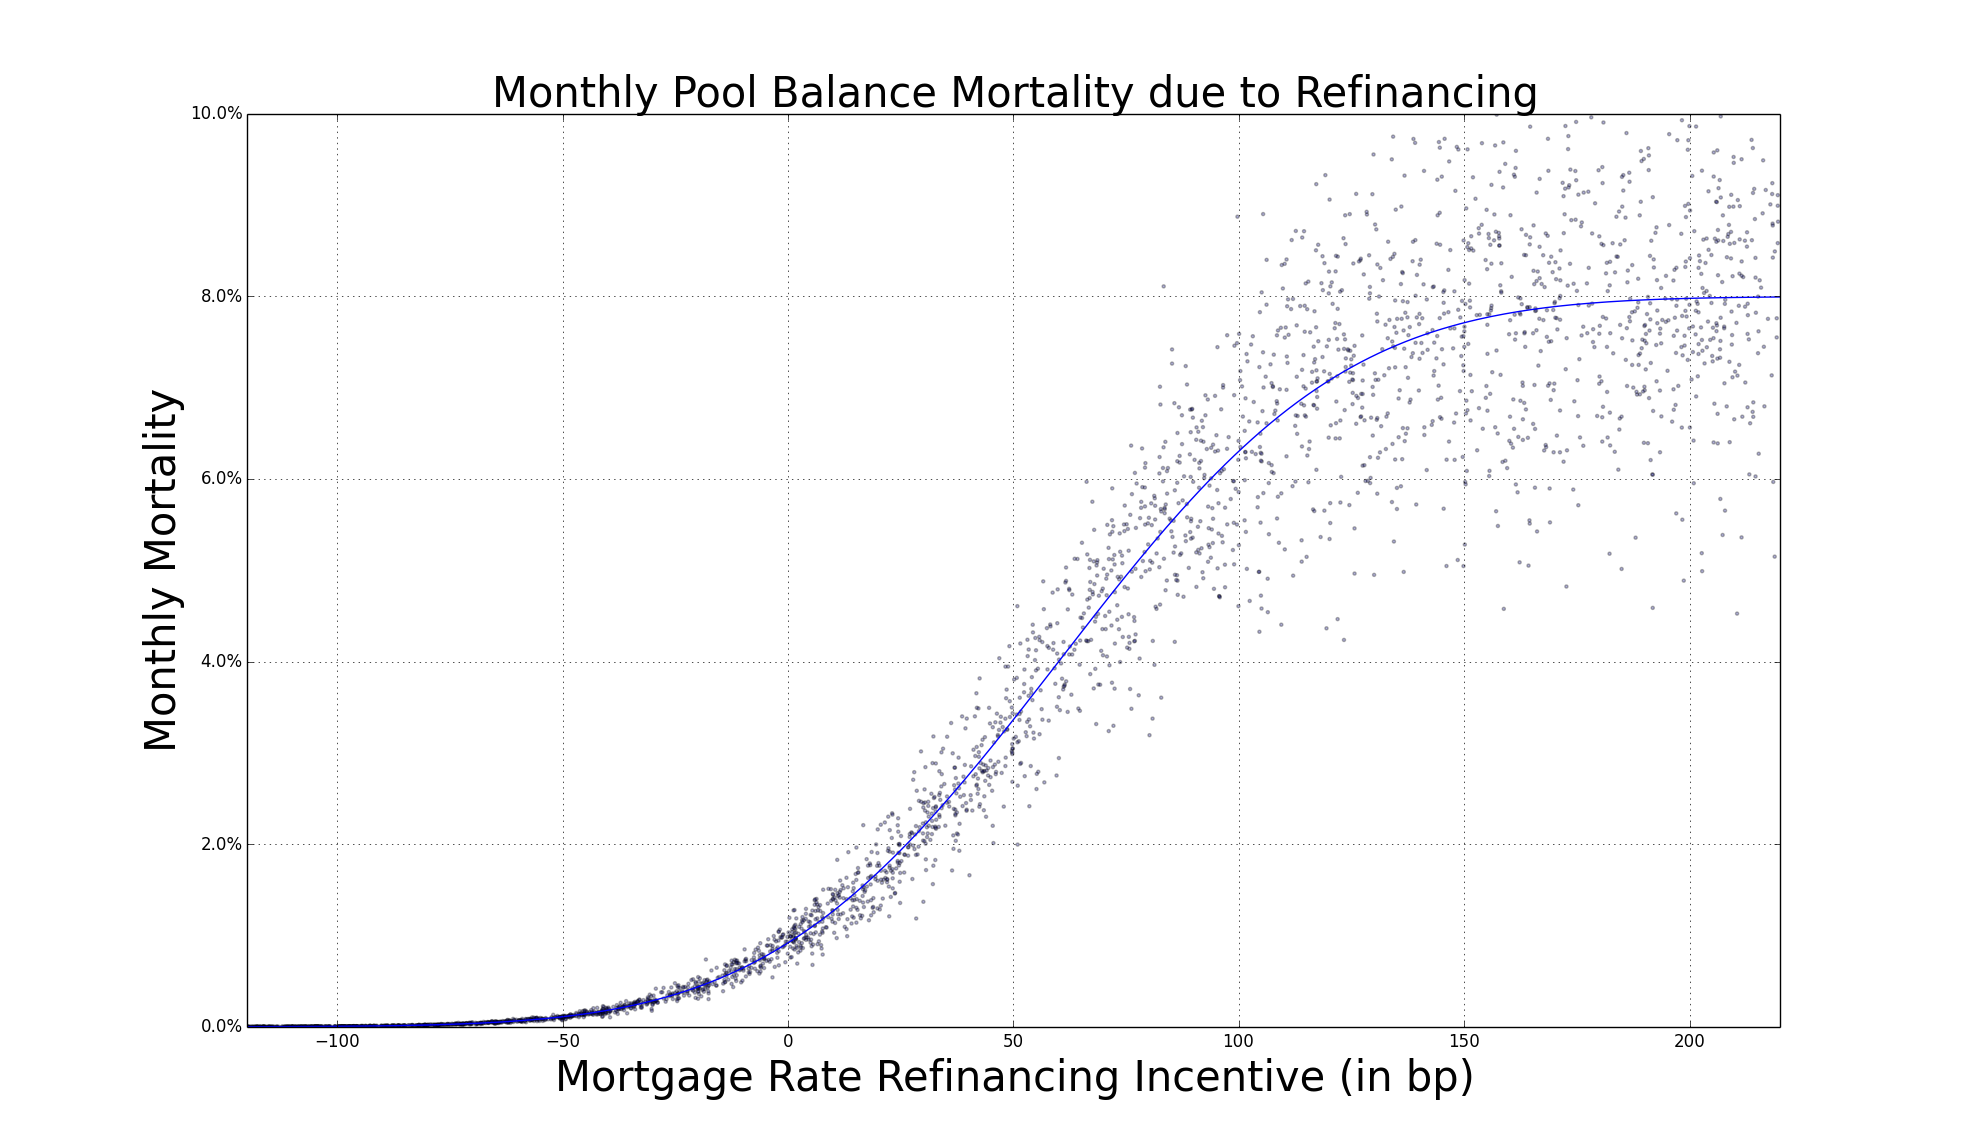
\includegraphics[scale=0.26]{refi_scurve.png}
\end{frame}

\begin{frame}
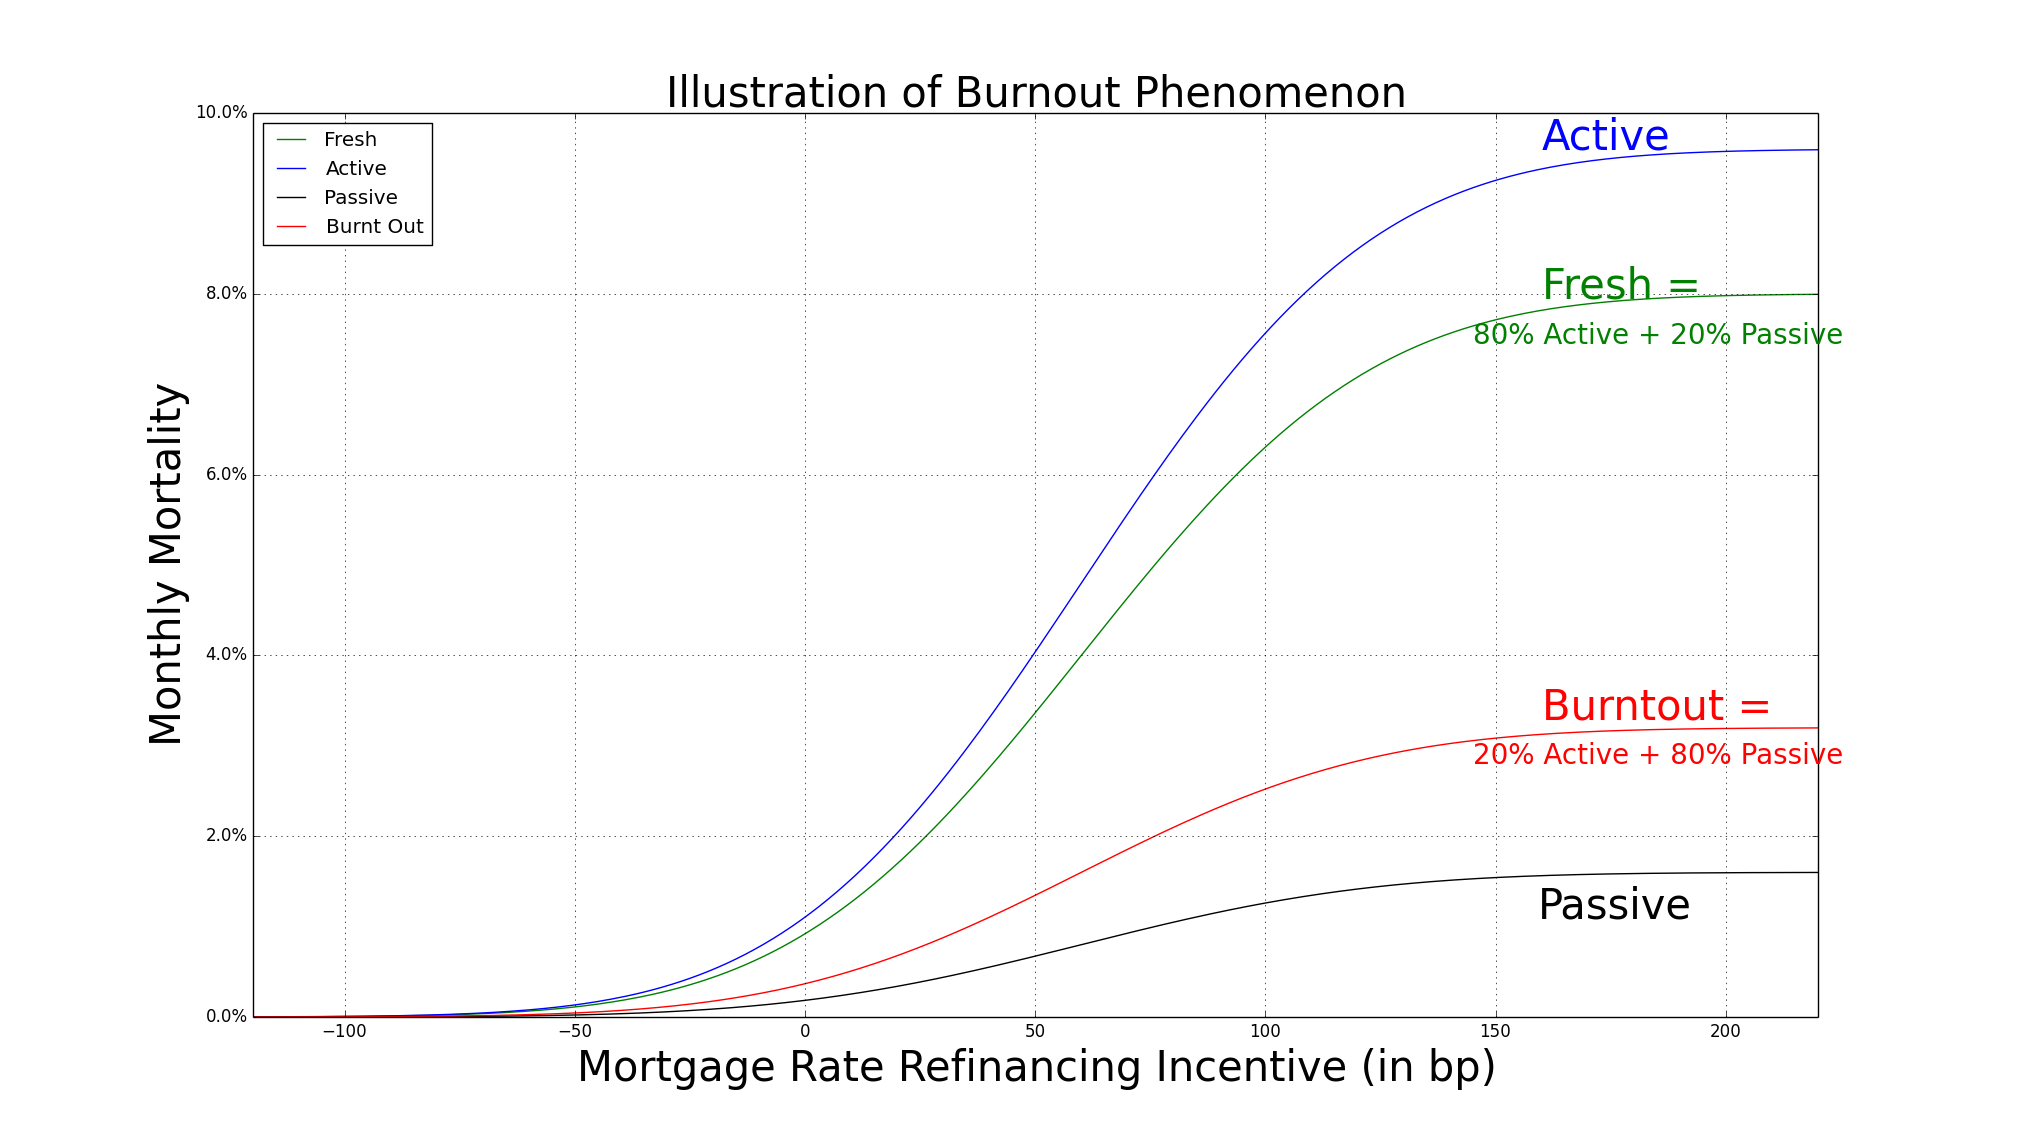
\includegraphics[scale=0.25]{burnout.png}
\end{frame}

\begin{frame}
\frametitle{Regression model of mortgage rates}
\begin{itemize}
\item Prepayment model typically based on mortgage rate ``moneyness''
\item Current Coupon (CC) model and Primary-Secondary Spread Model
\item Historical CC regressed against historical rates and vol
\item Instead, one can regress pricing-generated CC against rates and vol
\item But then this CC model is input to pricing
\item This fixed point is resolved by iterating to convergence
\item Alternative approach: Price Moneyness and Backward Induction
\end{itemize}
\end{frame}


\subsection{Challenges with Trading based on ``OAS''}
\begin{frame}
\frametitle{Pricing/Sensitivities based on ``Option-Adjusted Spread'' (OAS)}
If $T$ is maturity in months and $N$ is number of MC paths, 
$$Price = \frac 1 N \sum_{i=1}^N \sum_{t=1}^T (Principal_{i,t} + Interest_{i,t}) \cdot e^{-\sum_1^t (r_{i,u} + OAS)}$$
\begin{itemize}
\item OAS is a constant spread across time steps and MC paths
\item {\bf Risk-Premium for all risk factors other than interest rates}
\item Includes non-interest-rates prepayment risk, credit and liquidity risks
\end{itemize}

Pricing/Hedging with this OAS-based (industry-standard) approach:

\begin{itemize}
\item For MBS with market prices, assess rich/cheap based on implied OAS
\item For illiquid MBS, compute Price from trader-defined(!) OAS
\item Price Sensitivities (duration, convexity, vega) with constant OAS
\end{itemize}
\end{frame}

\begin{frame}
\frametitle{Significant challenges in Trading based on OAS}
\begin{itemize}
\item Passthrough MBS exhibit an ``OAS smile''
\item Empirical Duration performs better than Model Duration
\item Ill-formed theories on ``OAS Directionality''
\item IOs/POs from same collateral have vastly different OAS
\item IO Duration + PO Duration $\neq$ Underlying Pool Duration
\item Unclear what OAS to set to price illiquid MBS
\end{itemize}
{\bf We discuss an alternative approach for MBS Pricing based on:}
\begin{itemize}
 \item a continuous-cashflow PDE (and martingale) foundation
 \item Price of prepayment risk {\em modulo interest rate dependency}
 \item separating out residual non-prepayment risks (credit, liquidity)
 \end{itemize}
\end{frame}

\begin{frame}
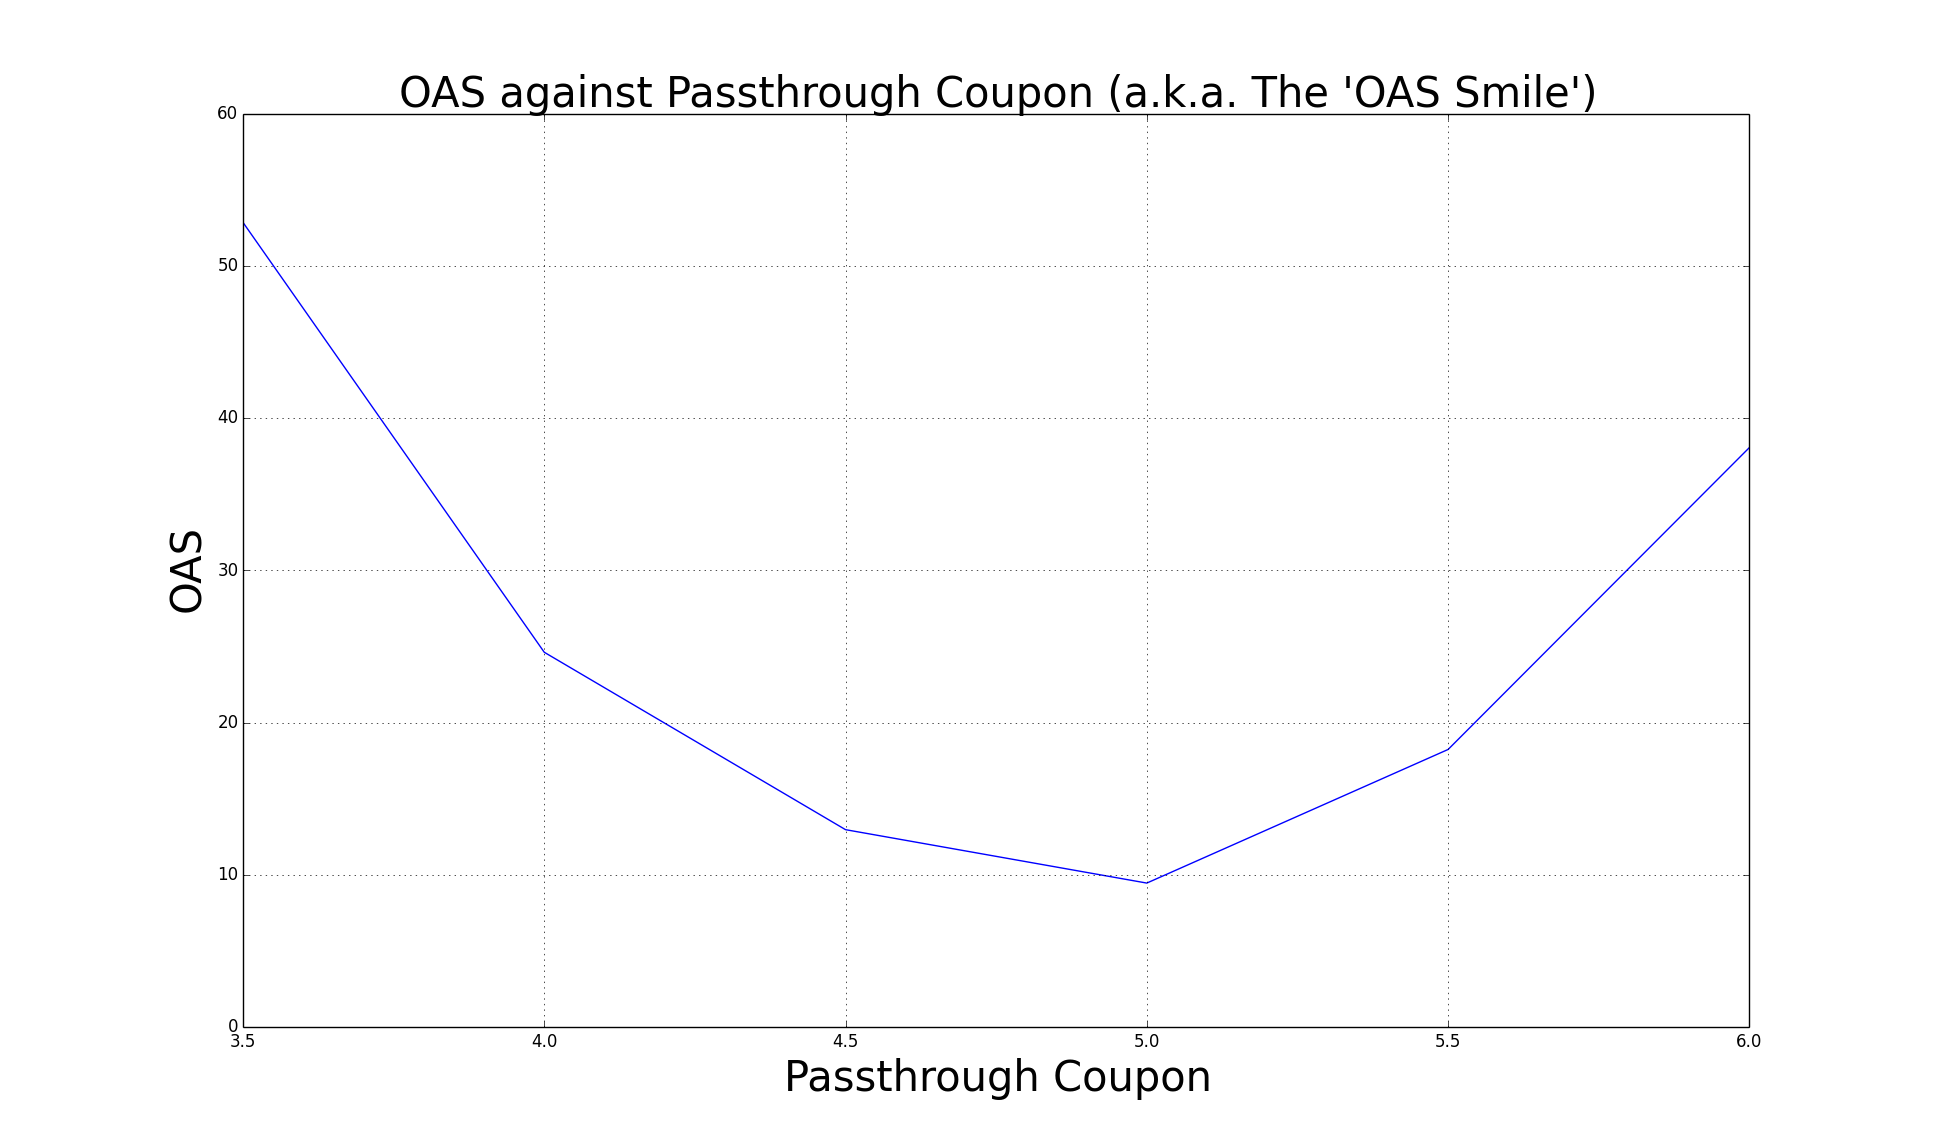
\includegraphics[scale=0.25]{oas_smile.png}
\end{frame}

\section{Alternative Formulations (to overcome challenges in trading)}
\subsection{Foundation 1: Continuous-Cashflow Pricing PDE}

\begin{frame}
\frametitle{Derivation of Continuous-Cashflow Pricing PDE}
Assume continuous-time cash flows and a 1-factor short-rate model.
$$ dr(t) = \alpha(r, t) \cdot dt + \sigma(r, t) \cdot dz(t)$$
\begin{itemize}
\item $B(t)$ is Balance, $P(t)$ is Price
\item $V(t) = P(t) \cdot B(t)$ is ``Value''
\item $c(r,t)$ is Coupon (interest paid per unit balance per unit time)
\item $\pi(r,t)$ is principal paid per unit balance per unit time
\end{itemize}
$$\pi(r,t) = sched(t) + sale(r,t) + refi(r,t) + curtail(r,t) + defaults(r,t)$$
Cashflow over time $dt$ is $(c(r,t) + \pi(r,t)) \cdot B(t) \cdot dt$
$$dB(t) = - \pi(r,t) \cdot B(t) \cdot dt$$
{\bf $\pi(r,t)$ is uncertain for fixed $r$ and $t$, but first assume it is certain}

\end{frame}

\begin{frame}
\frametitle{Derivation of Continuous-Cashflow Pricing PDE}
Consider two different MBS with notation subscripted with ``1'' and ``2''.
$$dV_1 = B_1 dP_1 + P_1 dB_1$$
Ito's Lemma for $dP_1$ and substituting $dB_1 = -\pi_1 B_1 dt$ gives:
$$dV_1 = B_1 (\pderiv{P_1}{t} dt + \pderiv{P_1}{r} dr + \frac {1} {2} \sigma^2 \pderiv[2]{P_1}{r} dt) - P_1 \pi_1 B_1 dt$$
$$ = B_1 (\pderiv{P_1}{t} + \alpha \pderiv{P_1}{r} -\pi P_1 + \frac {1} {2} \sigma^2 \pderiv[2]{P_1}{r}) dt + B_1 \sigma \pderiv{P_1}{r} dz$$

\begin{equation}
\frac {dV_1} {V_1} = (\frac {1} {P_1} \pderiv {P_1} {t}  + \frac {\alpha} {P_1} \pderiv{P_1}{r} -\pi_1 + \frac {\sigma^2} {2P_1} \pderiv[2]{P_1}{r})dt + (\frac {\sigma} {P_1} \pderiv{P_1}{r}) dz\label{eq:value-ito}
\end{equation}

\end{frame}

\begin{frame}
\frametitle{Derivation of Continuous-Cashflow Pricing PDE}
Denote the Ito drift and dispersion of $\frac {dV_1}{V_1}$ as $\alpha_1$ and $\sigma_1$.
\begin{equation}
\frac {dV_1} {V_1} = \alpha_1 dt + \sigma_1 dz
\end{equation}
\begin{equation}
\alpha_1 = \frac {1} {P_1} \pderiv {P_1} {t}  + \frac {\alpha} {P_1} \pderiv{P_1}{r} -\pi_1 + \frac {\sigma^2} {2P_1} \pderiv[2]{P_1}{r} \label{eq:drift}
\end{equation}
\begin{equation}
\sigma_1 = \frac {\sigma} {P_1} \pderiv{P_1}{r} \label{eq:dispersion}
\end{equation}

Consider a portfolio $W = V_1 + V_2 = P_1 B_1 + P_2 B_2$ with values of $B_1$ and $B_2$ such that we can eliminate the $dz$ term in the expression for $dW$
\begin{equation}
B_1 \pderiv{P_1}{r} = - B_2 \pderiv{P_2}{r} \label{eq:balances}
\end{equation}

Since we have eliminated the $dz$ term, portfolio $W$ together with the cashflow it generates should grow at the risk-free rate $r$. In other words,

$$dV_1 + dV_2 + B_1(c_1 + \pi_1) dt + B_2(c_2 + \pi_2) dt = r (V_1 + V_2) dt$$
\end{frame}

\begin{frame}
\frametitle{Derivation of Continuous-Cashflow Pricing PDE}
Expanding this out,
$$B_1(\pderiv{P_1}{t} + \alpha_1 \pderiv{P_1}{r} - \pi_1 P_1 + (c_1 + \pi_1) + \frac {\sigma^2}{2} \pderiv[2]{P_1}{r})dt + $$
$$B_2(\pderiv{P_2}{t} + \alpha_2 \pderiv{P_2}{r} - \pi_2 P_2 + (c_2 + \pi_2) + \frac {\sigma^2}{2} \pderiv[2]{P_2}{r})dt  = r(B_1P_1 + B_2P_2) dt$$

Combining this with equation \ref{eq:balances}, we get:

$$\frac{\pderiv{P_1}{t} + \alpha_1 \pderiv{P_1}{r} - (\pi_1 + r) P_1 + (c_1 + \pi_1) + \frac {\sigma^2}{2} \pderiv[2]{P_1}{r}} {\pderiv{P_1}{r}} = $$
$$\frac{\pderiv{P_2}{t} + \alpha_2 \pderiv{P_2}{r} - (\pi_2 + r) P_2 + (c_2 + \pi_2) + \frac {\sigma^2}{2} \pderiv[2]{P_2}{r}} {\pderiv{P_2}{r}}$$
\end{frame}

\begin{frame}
\frametitle{Derivation of Continuous-Cashflow Pricing PDE}
Using equations \ref{eq:drift} and \ref{eq:dispersion}, the above equation can be expressed as:

\begin{equation}
\frac{\alpha_1 + \frac{c_1 + \pi_1} {P_1} - r} {\sigma_1} = \frac{\alpha_2 + \frac{c_2 + \pi_2} {P_2} - r} {\sigma_2} \label{eq:sharperatio}
\end{equation}

\begin{itemize}
\item Note the numerator of LHS of Eq \ref{eq:sharperatio} is the expected {\em excess return} per unit time of investing in MBS 1 (expected growth rate of process $V_1$ together with its P \& I cash flows, less $r$).
\item The denominator is the standard deviation of the return per unit time.
\item Their ratio is the familiar {\bf Price of Interest-Rate Risk $\lambda_r$} (which is the same for every security exposed to only interest-rate risk).
\item This is what equation \ref{eq:sharperatio} is telling us, which can be re-expressed as:
\end{itemize}

$$\frac{\alpha_1 + \frac{c_1 + \pi_1} {P_1} - r} {\sigma_1} = \frac{\alpha_2 + \frac{c_2 + \pi_2} {P_2} - r} {\sigma_2} = \lambda_r$$

\end{frame}

\begin{frame}
\frametitle{Derivation of Continuous-Cashflow Pricing PDE}

Substituting in the above equation for $\alpha_1$ from equation \ref{eq:drift} and for $\sigma_1$ from equation \ref{eq:dispersion}, we get:

$$\frac{\frac {1} {P_1} \pderiv {P_1} {t}  + \frac {\alpha} {P_1} \pderiv{P_1}{r} -\pi_1 + \frac {\sigma^2} {2P_1} \pderiv[2]{P_1}{r} + \frac{c_1 + \pi_1} {P_1} - r} {\frac {\sigma} {P_1} \pderiv{P_1}{r}} = \lambda_r$$

Reorganize and drop the subscript $1$ in $P_1, c_1, \pi_1$ to arrive at the PDE:

$$\pderiv {P} {t}  + (\alpha - \lambda_r \sigma) \pderiv{P}{r}  + \frac {\sigma^2} {2} \pderiv[2]{P}{r} + c + \pi = (\pi + r)P$$

\end{frame}

\begin{frame}
\frametitle{Derivation of Continuous-Cashflow Pricing PDE}
If we shift to the risk-neutral measure (denoted as $Q$), $V_1$ together with the cash flows it generates should grow at risk-free rate $r$. Hence,

$$\frac {dV_1} {V_1} = (r - \frac {c_1 + \pi_1} {P_1})dt + \sigma_1 dz^{(Q)} = (\alpha_1 - \lambda_r \sigma_1) dt + \sigma_1 dz^{(Q)}$$

Since, $dz^{(Q)} = \lambda_r dt + dz$, the Ito process for the short-rate $r$ in the risk-neutral measure can be written as:

$$dr = (\alpha - \lambda_r \sigma) dt + \sigma dz^{(Q)} = \alpha^{(Q)} dt + \sigma dz^{(Q)}$$

where $\alpha^{(Q)} = \alpha - \lambda_r \sigma$ is the risk-neutral drift for $r$.

So, the PDE can also be expressed in terms of the risk-neutral drift of $r$:

$$\pderiv {P} {t}  + \alpha^{(Q)} \pderiv{P}{r}  + \frac {\sigma^2} {2} \pderiv[2]{P}{r} + c + \pi = (\pi + r)P $$
\end{frame}

\begin{frame}
\frametitle{Derivation of Continuous-Cashflow Pricing PDE}
\begin{itemize}
\item But in reality, $\pi$ depends on stochastic (risk) factors other than $r$
\item Each of which deserve a {\em Price of Risk} (hence, a return spread)
\item We cannot model/capture {\em Price of Risk} of all these factors. So,

$$\pderiv {P} {t}  + \alpha^{(Q)} \pderiv{P}{r}  + \frac {\sigma^2} {2} \pderiv[2]{P}{r} + c + \pi = (\pi + r + s)P \label{eq:pde1}$$
{\bf where $s$ is our ``good-old'' Option-Adjusted Spread (OAS).}

\item To unravel $s$, define stochastic factors for prepayments {\em other than $r$}
\item Not economic factors, but (multiplicative) {\bf forecast-error risk factors}
$$refi'(x,r,t) = refi(r,t) \cdot x(t)$$
$$sale'(y,r,t) = sale(r,t) \cdot y(t)$$
\end{itemize}
\end{frame}

\begin{frame}
\frametitle{Derivation of Continuous-Cashflow Pricing PDE}

$$dx(t) = \beta_x (1 - x) dt + \sigma_x dz_x(t) \mbox{ with } x(0) = 1$$
$$dy(t) = \beta_y (1 - y) dt + \sigma_y dz_y(t) \mbox{ with } y(0) = 1$$

Analogous to rate risk, shifting to risk-neutral measure, we have:
$$dx(t) = \alpha^{(Q)}_x dt + \sigma_x dz^{(Q)}_x(t) \mbox{ where } \alpha^{(Q)}_x = \beta_x (1 - x) - \lambda_x \sigma_x$$
$$dy(t)  = \alpha^{(Q)}_y dt + \sigma_y dz^{(Q)}_y(t) \mbox { where } \alpha^{(Q)}_y = \beta_y (1 - y) - \lambda_y \sigma_y$$

For consistency of notation, we define the risk-neutral process for $r$ as:

$$dr(t) = \alpha^{(Q)}_r dt + \sigma_y dz^{(Q)}_r(t)$$

Assume that the covariance of $dz^{(Q)}_x(t)$ and $dz^{(Q)}_y(t)$ is $\rho \cdot dt$ and that each of $dz^{(Q)}_x(t)$ and $dz^{(Q)}_y(t)$ are independent of $dz^{(Q)}_r(t)$. 

\end{frame}

\begin{frame}
\frametitle{Derivation of Continuous-Cashflow Pricing PDE}
\begin{equation}
\begin{split}
\pderiv {P} {t} & + \alpha^{(Q)}_r \pderiv{P}{r}  + \frac {\sigma_r^2} {2} \pderiv[2]{P}{r} + \alpha^{(Q)}_x \pderiv{P}{x}  + \frac {\sigma_x^2} {2} \pderiv[2]{P}{x} + \alpha^{(Q)}_y \pderiv{P}{y}  + \frac {\sigma_y^2} {2} \pderiv[2]{P}{y} \\
& + \rho \sigma_x \sigma_y \frac{\partial^2 P}{\partial x \partial y} + c + \pi^{(Q)} = (\pi^{(Q)} + r + rs)P \label{eq:pde2}
\end{split}
\end{equation}

\begin{itemize}
\item $Q$ now refers to risk-neutral measure with respect to joint $\{r,x,y\}$
\item $\sigma_x, \sigma_y, \rho, \beta_x, \beta_y$ estimated from errors in prepayment forecasts
\item $\lambda_x, \lambda_y$ calibrated to liquid MBS market prices (shifting $x,y$ drifts)
\item We refer to $Q$-measure-shifted $x, y$ ({\bf and $\pi^{(Q)}$}) as ``risk-neutral''
\item $rs$ is the spread due to any residual risk such as liquidity or credit
\item {\bf $s - rs$ due to prepayment risk modulo interest rates dependency}
\end{itemize}

\end{frame}

\begin{frame}
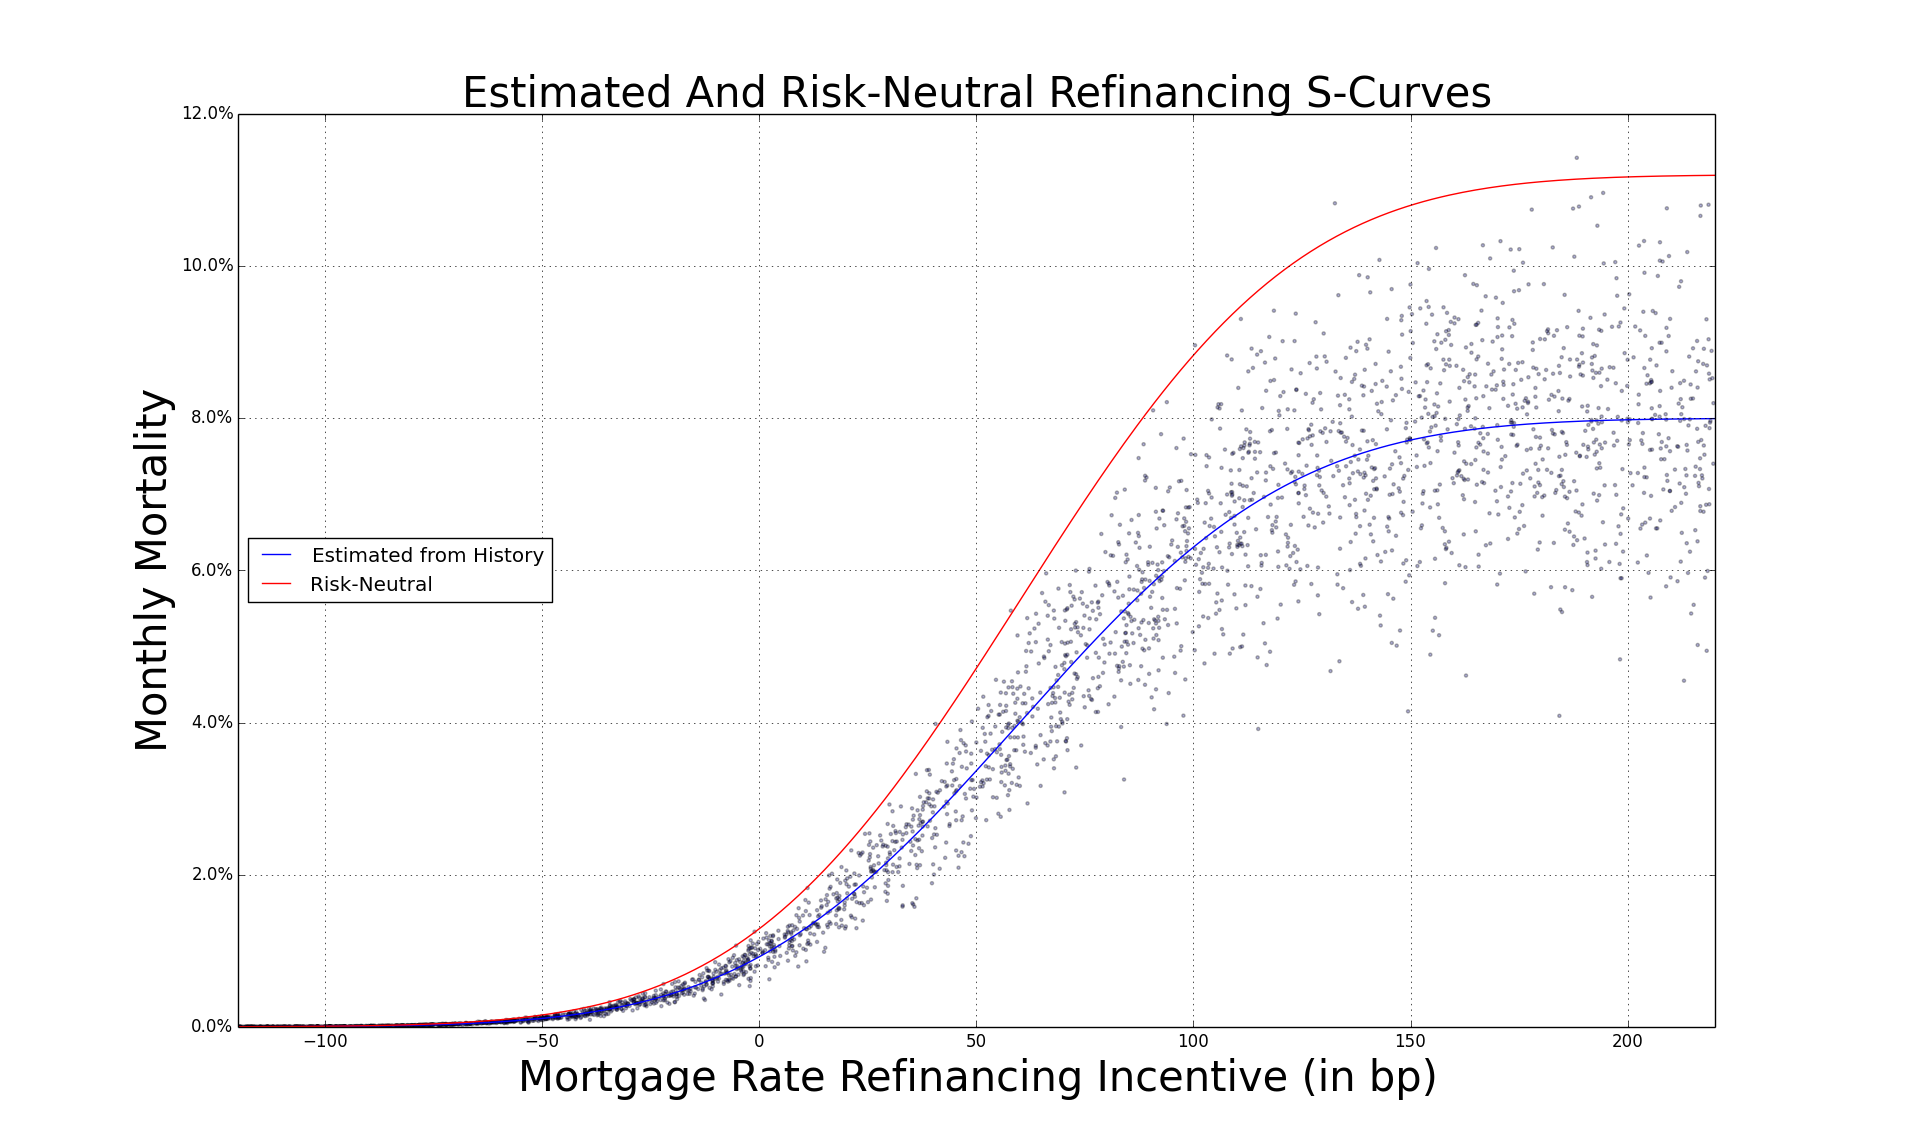
\includegraphics[scale=0.27]{risk_neutral_scurve.png}
\end{frame}

\begin{frame}
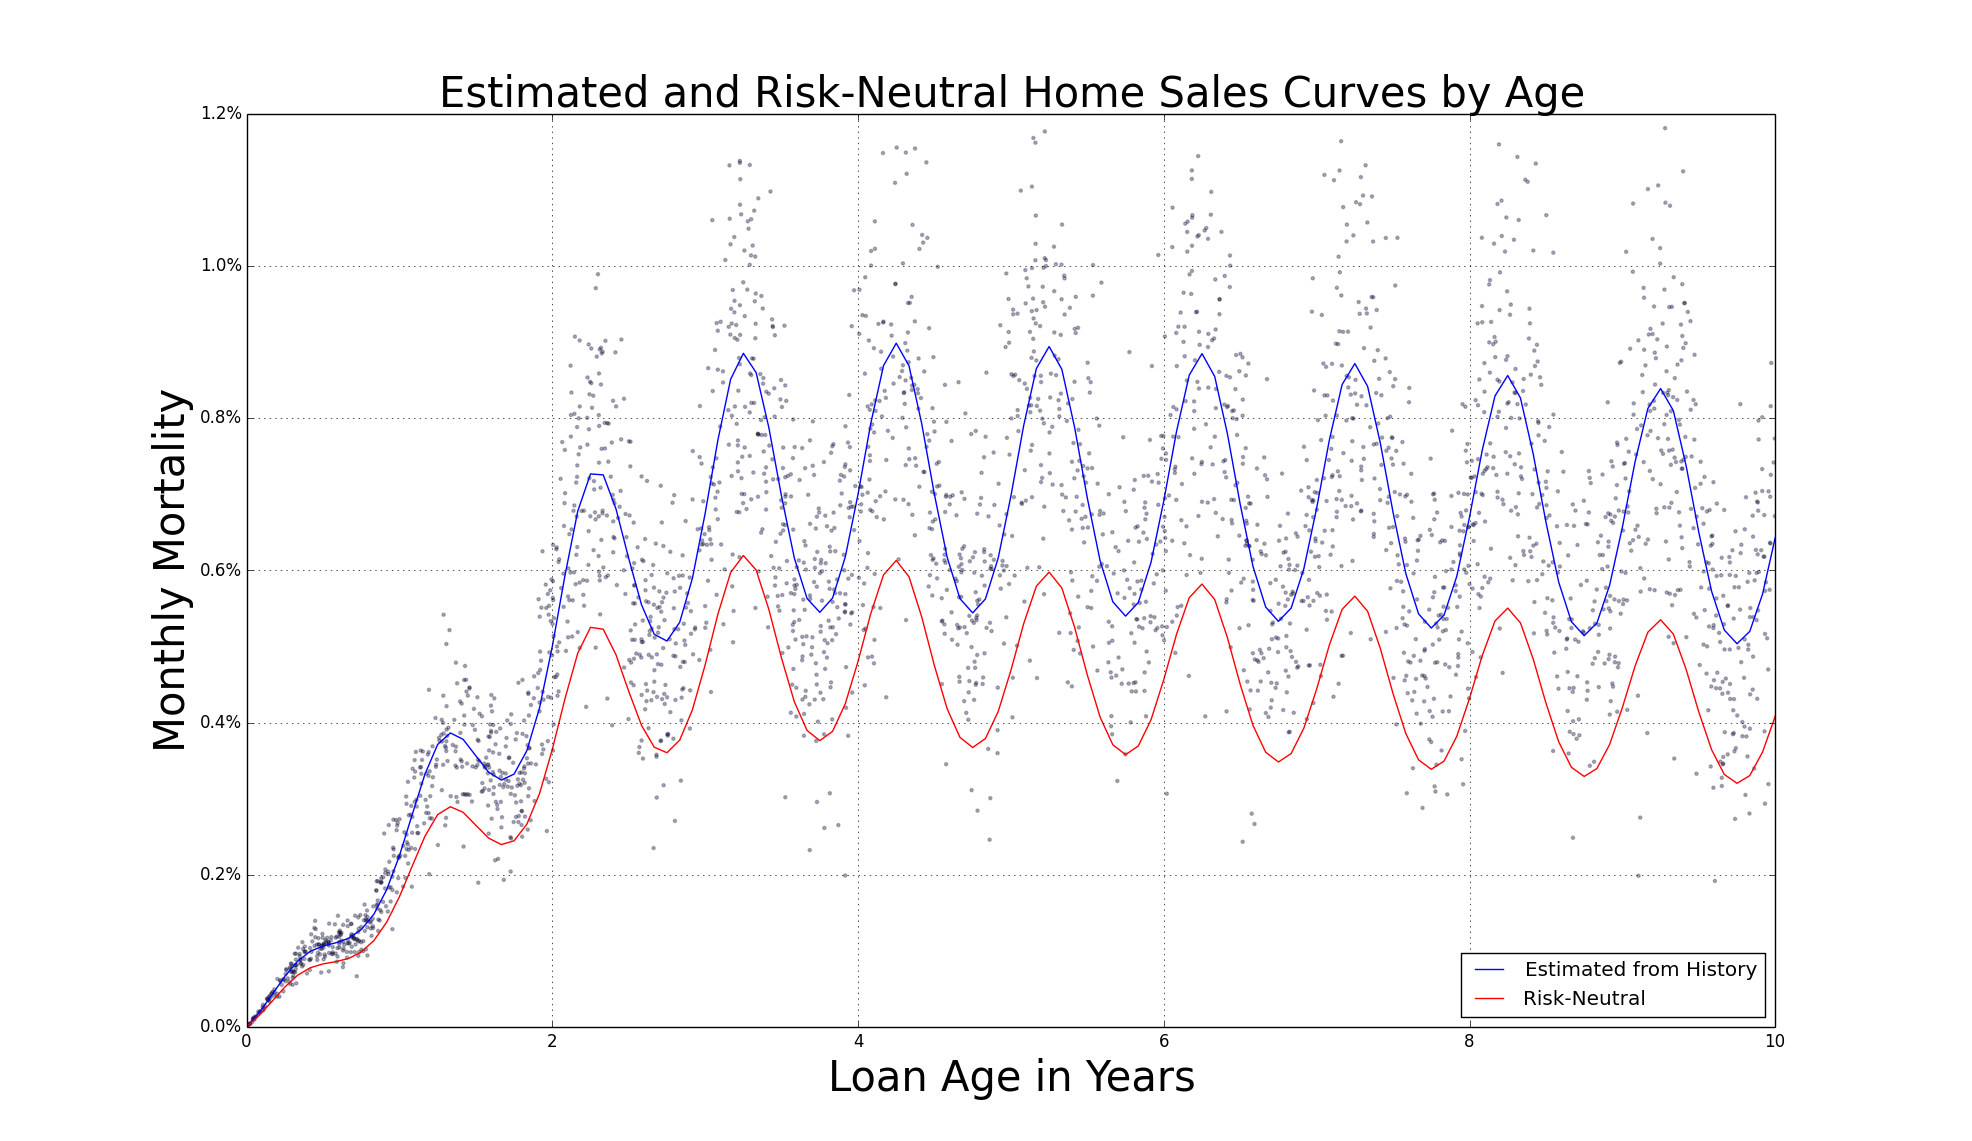
\includegraphics[scale=0.26]{risk_neutral_relo.png}
\end{frame}



\subsection{Foundation 2: Expected Discounted Cashflow (EDC) Pricing Formula}

\begin{frame}
\frametitle{Martingale-based (Expected Discounted Cashflow) Pricing}
Define the money-market process $M(t)$ as:

$$dM(t) = r(t) \cdot M(t) \cdot dt, M(0) = 1$$

Consider a process $\theta(t)$ derived from $V(t)$ and the cash flows, as follows:

$$d\theta(t) = dV(t) + (c(r,t) + \pi(r,t)) B(t) dt$$

As before, assume $\pi(r,t)$ is certain for fixed $r$. Then, $\frac {\theta(t)} {M(t)}$ is a martingale in risk-neutral measure $Q$. So, for any $T > 0$,

$$\frac {\theta(0)} {M(0)} = E_Q[\frac {\theta(T)} {M(T)}]$$

Since $\theta(0) = V(0), M(0) = 1$, and without loss of generality, $B(0) = 1$,

$$P(0) = \frac {\theta(0)} {M(0)} = E_Q[\frac {V(T) + \int_0^T (c(r,t) + \pi(r,t))\cdot B(t) \cdot dt} {M(T)}]$$

\end{frame}

\begin{frame}
\frametitle{Martingale-based (Expected Discounted Cashflow) Pricing}

If we set $T$ to MBS maturity, $V(T) = B(T) = 0$. Then,

\begin{equation}
\begin{split}
P(0) & = E_Q[\int_0^T \frac {(c(r,t) + \pi(r,t)) \cdot B(t)} {M(t)} dt] \\
& = E_Q[\int_0^T (c(r,t) + \pi(r,t)) \cdot B(t) \cdot e^{-\int_0^u r(u) du} dt] \\
& = E_Q[\int_0^T (c(r,t) + \pi(r,t)) \cdot e^{-\int_0^u (r(u) +\pi(r, u)) du} dt]
\end{split}
\end{equation}
{\bf Conceptualize as cash flows discounted at rate $r + \pi$ in $Q$-measure}
\end{frame}

\begin{frame}
\frametitle{Martingale-based (Expected Discounted Cashflow) Pricing}
\begin{itemize}
\item But in reality, $\pi$ depends on stochastic (risk) factors other than $r$
\item Each of which deserve a {\em Price of Risk} (hence, a return spread)
\item We cannot model/capture {\em Price of Risk} of all these factors. So,
\end{itemize}
\begin{equation}
\begin{split}
P(0) & = E_Q[\int_0^T (c(r,t) + \pi(r,t)) \cdot B(t) \cdot e^{-\int_0^u (s + r(u)) du} dt] \\
& = E_Q[\int_0^T (c(r,t) + \pi(r,t)) \cdot e^{-\int_0^u (s + r(u) + \pi(r, u)) du} dt]
\end{split}
\end{equation}

Introducing multipliers $x, y$ and calibrating $\lambda_x, \lambda_y$ to liquid MBS prices, we denote the resulting principal payment rate as $\pi^{(Q)}(x,y,r,t)$:

\begin{equation}
\begin{split}
P(0) & = E_Q[\int_0^T (c + \pi^{(Q)}) \cdot B(t) \cdot e^{-\int_0^u (rs + r(u)) du} dt] \\
& = E_Q[\int_0^T (c + \pi^{(Q)}) \cdot e^{-\int_0^u (rs + r(u) + \pi^{(Q)}) du} dt]\label{eq:martingale}
\end{split}
\end{equation}
\end{frame}

\begin{frame}
\frametitle{Alternative approaches to Pricing/Sensitivity Computations}
\begin{itemize}
\item Closed-form approximations for pricing and price sensitivities
\item Pricing on a grid (Markovian)
\item Pricing and Hedging based on ``risk-neutral prepayments'' and residual spread (instead of OAS).
\end{itemize}
\end{frame}

\subsection{Closed-Form Approximations for Price and Sensiivities}

\begin{frame}
\frametitle{Closed-Form Approximations for Price and Sensitivities}
\begin{itemize}
\item Closed-form Solution for Expected Discounted Cashflow (EDC) formula when $\pi(r,t) = \pi_0(t) + r \pi_1$ and $c(r,t) = c_0(t) + r \cdot c_1(t)$
\item Closed-form Solution for Pricing PDE when $r$ follows an affine process and $\pi(r,t) = \pi_0(t) + r \pi_1$ and $c(r,t) = c_0(t) + r \cdot c_1(t)$
\item Closed-form Solution for EDC Price formula when $\pi$ is linear in $r$ with hard max and min
\item The above gives bad greeks due to piecewise prepayment function. But this serves quite useful as a control variate.
\item We can do analytical partial derivatives of EDC Price formula w.r.t:
\begin{itemize}
\item a time-parallel shift to $r(t)$ (Duration approximation)
\item coupon $c$
\item a time-parallel shift to $\pi(r,t)$ (Prepayment sensitivity)
\item a time-parallel shift to refi multiplier $x(t)$ or sale multiplier $y(t)$
\item residual spread $rs$
\end{itemize}
\item {\bf These closed-forms very useful to reason about pricing/sensitivities}
\end{itemize}
\end{frame}

\subsection{Markovian Pricing (on a Grid) - simpler, cleaner, faster}

\begin{frame}
\frametitle{Markovian Pricing (on a Grid)}
\begin{itemize}
\item Model Burnout by creating a few (2-3) cohorts in the pool, each of which is homogeneous in terms of refinancing efficiency
\item {\bf Each cohort's prepayment incentive is Markovian}
\item For each cohort, at every grid node, probabilistically discount sum of:
\begin{itemize}
\item Interest cash flow $c$
\item Principal cash flow $\pi$
\item $(1 - \pi) \cdot P$
\end{itemize}
\item This gives a backward induction for $P$ for each cohort
\item MBS Price = sum of cohort Prices
\item Alternatively, we can solve Pricing PDE with Crank-Nicholson
\item Making $\pi$ a function of $P$ (instead of $r$) yields a clean model
\end{itemize}
Caveat: ARMs and some CMOs have non-Markovian cash flows.
\end{frame}

\subsection{{\bf Proposal: Pricing/Hedging with  ``risk-neutral prepayments''}}

\begin{frame}
\frametitle{Pricing and Hedging with ``risk-neutral prepayments''}
Trading with ``risk-neutral prepayments'' and residual spread $rs$
\begin{itemize}
\item For MBS with market prices, assess rich/cheap based on implied $rs$
\item For illiquid MBS, Price using a prudent $rs$ (easier than a OAS input)
\item Price Sensitivities {\bf using constant rs} (instead of constant OAS)
\end{itemize}
\end{frame}

\begin{frame}
\frametitle{Practical considerations in designing the Pricer}
\begin{itemize}
\item I used TBA prices for calibration (liquid IOs/POs could also be used)
\item I calibrated Price of Risk of uncertain initial values $x(0)$ and $y(0)$, along with Price of Risk of $dz_x, dz_y$
\item I set $rs =$ Agency-Swap spread plus appropriate liquidity spread \\ (we can do better by building a proper model for residual risk)
\item {\bf Small $\pderiv[2]{P}{x}, \pderiv[2]{P}{y} \Rightarrow $ we can avoid stochasticity of $x, y$ in Pricer}
\item So calibrated $\alpha_x^{(Q)}, \alpha_y^{(Q)}$ essentially give us $E_Q[x(t)], E_Q[y(t)]$
\item This gives us a (deterministic) shifted prepayment function $\pi^{(Q)}(r,t)$
\item {\bf Practically, use same old Pricer, simply alter $\pi(r,t)$ to $\pi^{(Q)}(r,t)$}
\end{itemize}
\end{frame}

\begin{frame}
\frametitle{Are we happy? Can we improve?}
\begin{itemize}
\item ``OAS Smile'' captured (but sometimes small residual smile remains)
\item Model Durations match Empirical (``OAS Directionality'' captured)
\item Model prices for IOs/POs are fairly close to their market prices
\item IOs: $rs$-based Duration more negative than OAS-based Duration 
\item Superior hedge performance relative to OAS-based Duration
\item Further work (will help in crisis periods) - make $rs$ a function of:
\begin{itemize}
\item General credit risk
\item Agency-specific credit risk
\item Supply/Demand-based liquidity risk
\end{itemize}
\item Modeling $x,y$ as a jump-diffusion would also be a good idea 
\end{itemize}
\end{frame}

\begin{frame}
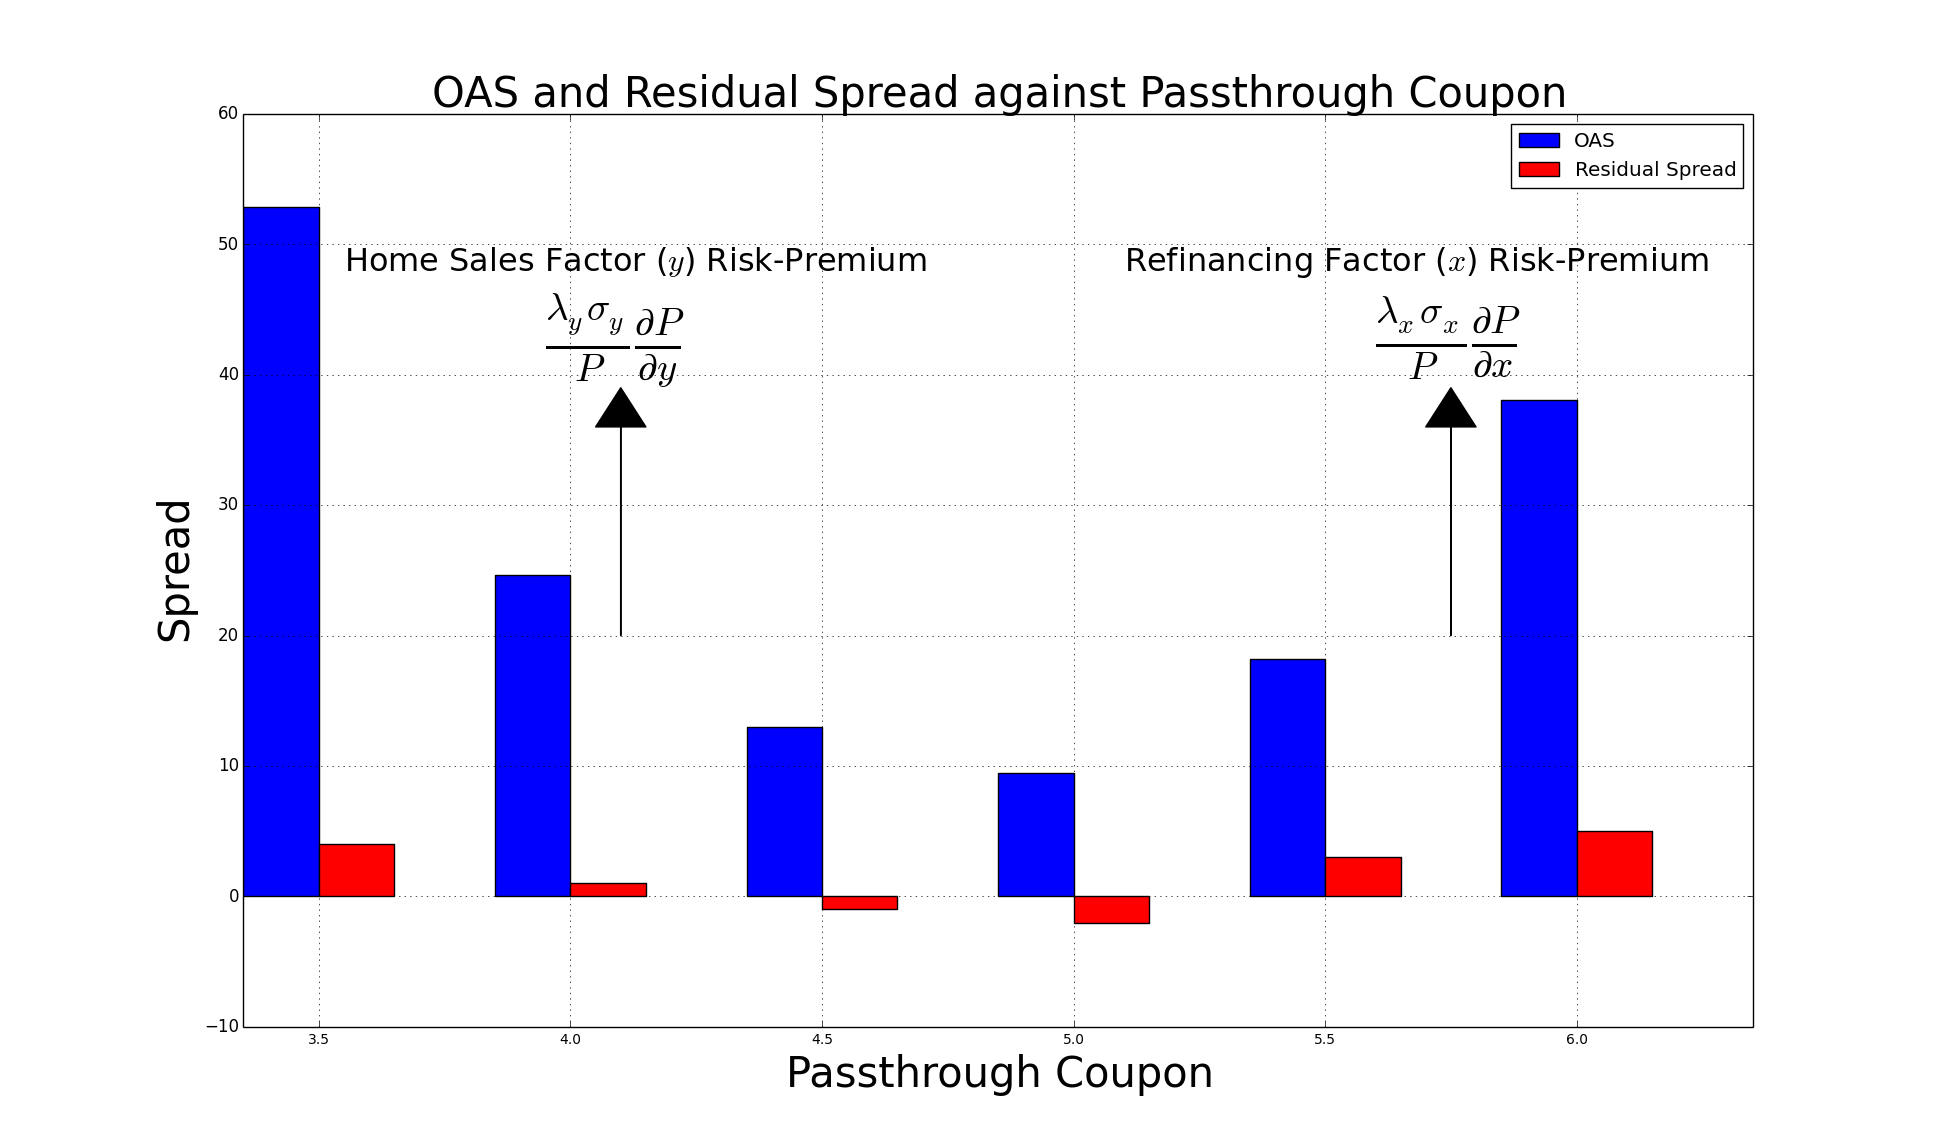
\includegraphics[scale=0.27]{oas_smile_rs_smile.png}
\end{frame}

\begin{frame}
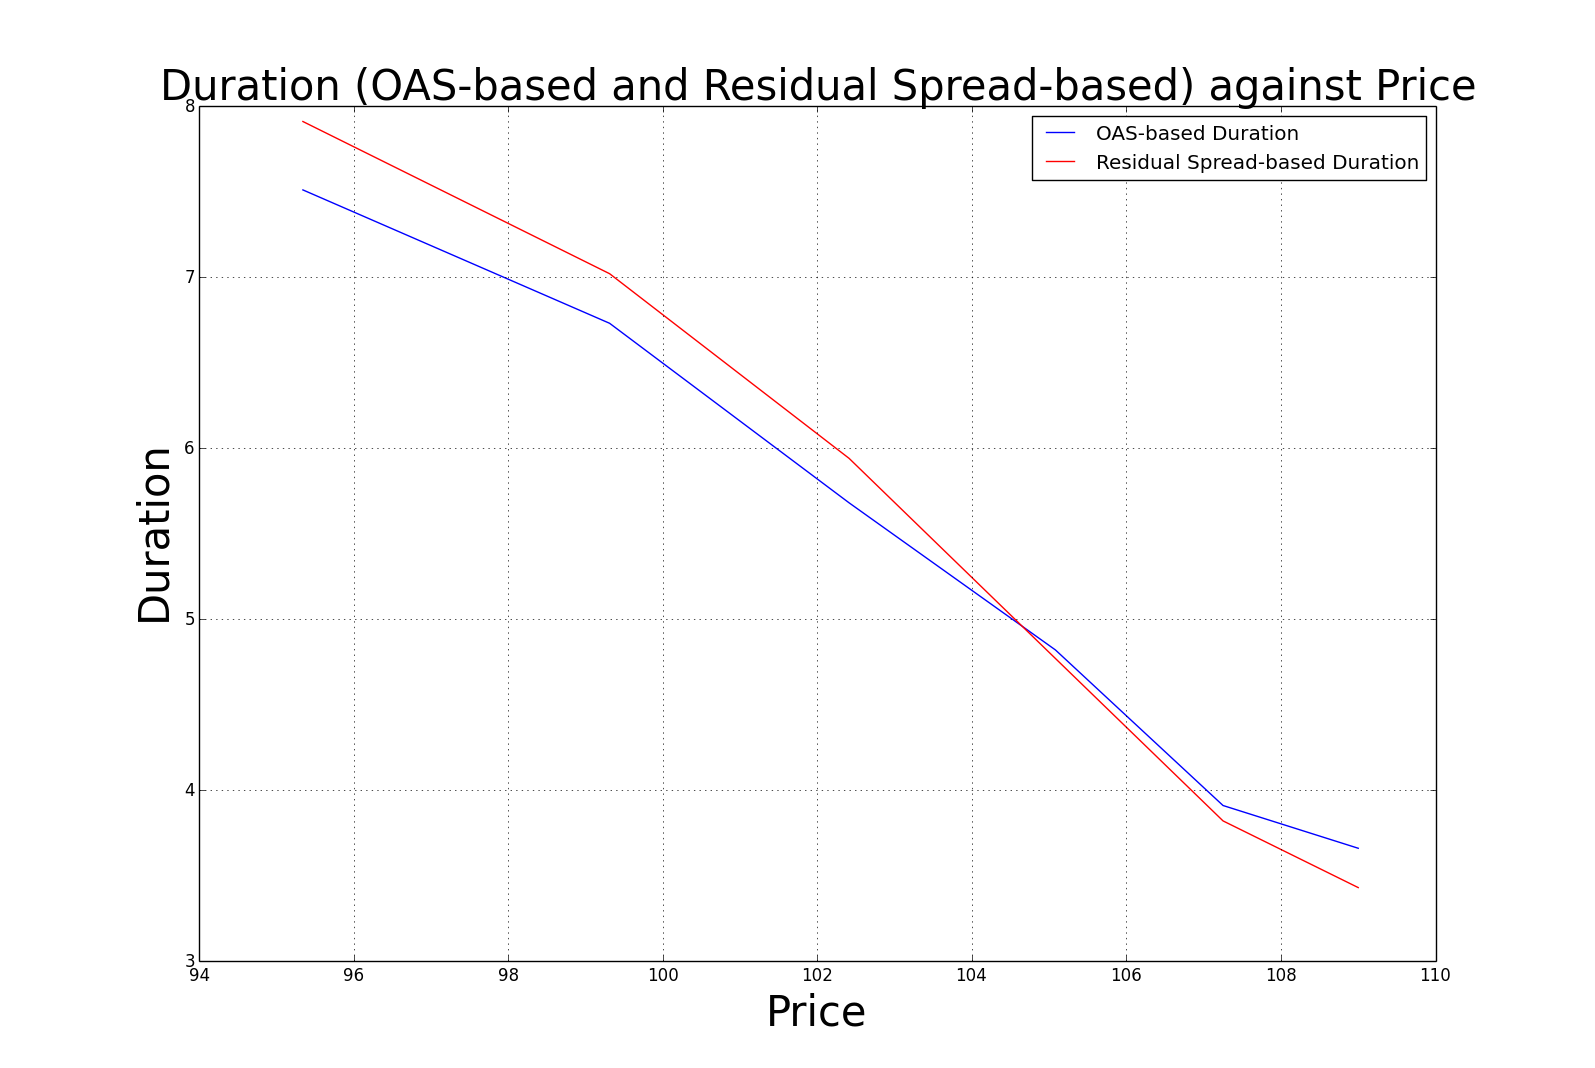
\includegraphics[scale=0.32]{oas_dur_rs_dur.png}
\end{frame}

\begin{frame}
\frametitle{Appendix: Sign of Price of Risk}
For risk factor $f$, the vol of $\frac {dV} {V}$ w.r.t $f$ is $\frac {\sigma_f} {P} \pderiv{P}{f}$.\\
So the risk-premium (spread) for the MBS due to the risk factor $f$ is:
$$\frac {\lambda_f \sigma_f} {P} \pderiv{P}{f}$$

\begin{itemize}
\item We calibrate $\lambda_x$ and $\lambda_y$ to liquid passthrough market prices
\item Premiums are mainly exposed to refinancing risk and $\pderiv{P}{x}$ is negative
\item OAS smile $\Rightarrow \lambda_x$ (Price of Refinancing-Forecast Risk) is negative
\item Discounts are mainly exposed to home sales risk and $\pderiv{P}{y}$ is positive
\item OAS smile $\Rightarrow \lambda_y$ (Price of HomeSales-Forecast Risk) is positive
\end{itemize}
\end{frame}

\begin{frame}
\frametitle{Appendix: Direction of risk-neutral adjustment of drift}
For risk factor $f$, it's drift is subtracted by $\lambda_f \sigma_f$ to make the process for $f$ risk-neutral. Risk-premium $s$ due to the risk factor $f$ is given by:

$$s = \frac {\lambda_f \sigma_f} {P} \pderiv{P}{f} $$

So, the drift of $f$ is subtracted by:

$$\frac{sP} {(\pderiv{P}{f})}$$

\begin{itemize}
\item $s > 0 \Rightarrow$ drift is adjusted in a direction that worsens price
\item So, adjusted Refinancing multiplier $E_Q[x(t)]  > 1$
\item And adjusted HomeSales multiplier $E_Q[y(t)] < 1$
\end{itemize} 
\end{frame}

\begin{frame}
\frametitle{Summary and Finishing Comments}
\begin{itemize}
\item ``Risk-Neutral Prepayments'' have been discussed since the mid-90s.
\item But practitioners shy away claiming ``Pricing Theory is not for MBS''!
\item I was first influenced to implement this by Alex Levin in 2006
\item My motivations: A) Improved Rich/Cheap, \& B) Hedge Performance
\item Despite frailties, I see the following as a big upgrade for Trading:\\
{\bf Deep Learning models layered with Price of Risk calibration}
\item Further work on residual Liquidity/Credit Risk (for times of crises!)
\item Can we extend this idea to non-Agency (default-risky) MBS?
\end{itemize}
\end{frame}

\end{document}